% 设置 biblatex 额外选项
% \PassOptionsToPackage{gbpub=false, gbtype=false}{biblatex}

% 载入 SJTUThesis 模版
% \documentclass[degree=doctor, zihao=-4, language=english, review]{sjtuthesis}
%\documentclass[degree=master, zihao=-4]{sjtuthesis}
\documentclass[degree=bachelor, openany, oneside]{sjtuthesis}
% \documentclass[degree=course, language=english, openright, twoside]{sjtuthesis}
% 选项
%   degree=[doctor|master|bachelor|course],     % 必选,学位类型
%   language=[chinese|english],                 % 可选(默认:chinese),论文的主要语言
%   bibstyle=[gb7714-2015|gb7714-2015ay|ieee],  % 可选(默认:gb7714-2015),参考文献样式
%   review,                                     % 可选(默认:关闭),盲审模式

% 所有其它可能用到的包都统一放到这里了,可以根据自己的实际添加或者删除。
\usepackage{sjtuthesis}
% \usepackage{graphicx} 
% \usepackage{subfigure}

% 定义图片文件目录与扩展名
\graphicspath{{figure/}}
\DeclareGraphicsExtensions{.pdf,.eps,.png,.jpg,.jpeg}

% 导入参考文献数据库
\addbibresource{bib/thesis.bib}

% 信息录入,必须在导言区进行!
% !TEX root = ../thesis.tex

%TC:ignore

\title{针对可扩展内存完整性保护的设计与实现}
\author{冯二虎}
\studentid{516030910082}
\supervisor{夏虞斌教授}
% \assisupervisor{某某教授}
\degree{本科}
\major{软件工程}
\department{电子信息与电气工程专业}
\date{2020年6月19日}
% \fund{国家 973 项目 (No. 2025CB000000) \\ 国家自然科学基金 (No. 81120250000)}
\keywords{完整性保护,内存控制器,计算机安全}

\entitle{SCALABLE MEMORY INTEGRITY PROTECTION DESIGN AND RESEARCH }
% \enauthor{erhu Feng}
% \ensupervisor{Prof. Mou Mou}
% % \enassisupervisor{Prof. Uom Uom}
% \endegree{Master of Engineering}
% \enmajor{A Very Important Major}
% \endepartment{Depart of XXX}
% \endate{Dec. 17th, 2014}
% \enfund{National Basic Research Program of China (Grant No. 2025CB000000) \\
%   National Natural Science Foundation of China (Grant No. 81120250000)}
\enkeywords{integrity protection, memory controller, computer security}

%TC:endignore


% 自定义项目标签名称
% \sjtuSetLabel{
%   listfigure = {图\quad 录},
%   listtable  = {表\quad 录}
% }

\begin{document}

% 无编号内容:中英文论文封面、授权页
\maketitle
% \makeDeclareOriginality[pdf/originality.pdf]
% \makeDeclareAuthorization

% 使用罗马数字对前言编号
\frontmatter

% 摘要
% !TEX root = ../thesis.tex

\begin{abstract}
内存保护是计算机安全中的重要组成部分,针对内存的攻击被划分为软件攻击与硬件攻击,软件攻击可以通过内存隔离防御,而硬件攻击需要通过内存加密与完整性保护来防御。
内存隔离和加密在计算机系统与安全中都有较为成熟的解决方式,但是内存完整性保护还面临着内存大小与性能之间的权衡。2016英特尔推出了Software Guard Extensions(SGX),
SGX能够实现内存隔离,加密与完整性保护,从而为enclave程序提供了可信执行环境。虽然SGX提供了强安全保障机制,但是enclave能够使用的内存仅仅只有128M,受限于内存的完整性保护。

在本文中,提出了一种新颖的可扩展内存完整性保护方案:挂载式完整性保护树。它能够保护TB级别的内存数据,实现离散的内存保护与动态的安全内存分配。同时,我们为完整性保护树提供了动态原语:挂载与卸载,以代替
SGX中采用的页交换机制,实现了可扩展的内存保护。

我们在gem5上实现了可挂载完整性保护树的原型,并且在SPECCPU上做了初步的测试。测试的结果表明,采用了可挂载完整性保护树相较于之前先进的VAULT和SIT提升了2~3
倍的性能,在极限的场景下能够提升7~8倍的性能。可挂载完整性保护树为可信执行环境,非易失性内存等新兴的应用场景与硬件提供了强安全保障,弥补了内存保护中,完整性保护的缺陷。

\end{abstract}

\begin{enabstract}
  Memory protection is an important part of computer security. Attacks against memory are divided into software attacks and hardware attacks. Software attacks can be defended by memory isolation, while hardware attacks need to be defended by memory encryption and integrity protection.

  Memory isolation and encryption have relatively mature solutions in computer systems and security, however memory integrity protection still face the trade-off between memory size and performance. In 2016, Intel launched the Software Guard Extensions (SGX), SGX enables memory isolation, encryption, and integrity protection, which provides a trusted execution environment for enclave. However although SGX provides strong security mechanism, enclave can only use 128M for memory, which is limited by memory integrity protection.
  
  In this paper, a novel scalable memory integrity protection scheme is proposed: Mountable Merkle tree (MMT), which can protect TB level memory data and realize discrete memory protection and dynamic secure memory allocation. At the same time, we provide dynamic primitives for integrity protection trees: mount and unmount, which can significantly improve the performance against the page swapping mechanism adopted in SGX. We implement a prototype of a mountable merkle tree on gem5 and do the preliminary testing on SPECCPU. The results of the tests show that using the mountable merkle tree can improve 2 to 3 times better performance compared to VAULT and SIT, and 7 to 8 times performance improvement in the extreme scenarios. Mount Merkle tree can provide robust memory security protection for the trusted execution environment, 
  non-volatile memory and other emerging scenarios and new hardware, and make up the integrity protection defects in traditional memory protection.
\end{enabstract}


% 目录、插图目录、表格目录
\tableofcontents
\listoffigures
\listoftables
% \listofalgorithms

% 主要符号、缩略词对照表
% \input{tex/nomenclature}

% 使用阿拉伯数字对正文编号
\mainmatter

% 正文内容
% !TEX root = ../thesis.tex

\chapter{概述}

\section{研究背景}
在数字化的当下,计算机安全越来越受到厂商与消费者们的关注,日益复杂的软件程序和各异的硬件平台暴露出了更多的安全隐患,其中与内存相关的攻击占了绝大多数。
基于内存的攻击可以分为两类:一类是软件攻击;另一类是硬件攻击。近年来研究者们通过新的硬件特性与软件架构,提出了诸多解决方案,其中内存完整性保护是不可或缺
的一点。内存的完整性保护机制保证了内存不会受到诸如修改、拼接、重放等物理攻击,提供了很强的安全保障。传统的完整性保护使用的是merkle tree,通过树状
结构,父节点中保存子节点的hash值,最后所有的数据将受到root hash的保护。 merkle hash发明以来受到广泛的应用,在文件系统、网络传输中起到了至关重要的作用
近几年,BMT,SIT等新的数据结构相继提出,尝试解决merkle tree存在的缺陷。

2016年,英特尔提出了Software Guard Extension(SGX),是第一个商用的可信执行环境并且提供了内存隔离,内存加密与内存完整性保护等强内存保护机制。SGX一经推出
就受到了学术界和工业界广泛的使用。虽然SGX提供了很强的安全保障,但是支持的内存只有128/256M,无法满足云场景下的需求,而限制SGX所保护内存大小的一个重要因素就是
内存完整性保护机制。在SGX中内存完整性保护的数据结构为Sgx Integrity Tree(SIT)。随着保护的内存增加,SIT的深度也随之增加,随之将带来严重的运行开销。SGX通过
限制SIT的深度(即限制了所保护内存的大小),来确保运行时的开销在一个可接受的范围内。 

在云计算普及的当下,计算机对内存的需求也越来越大,传统的merkle tree或者其变种无法支持在云场景下的TB级别的内存保护,2018年学术界提出了vault,用于扩展SIT所
保护的内存空间。虽然vault将受保护的内存扩大到了GB的量级,但是仍然无法满足云场景下的需求。另外所有的内存完整性保护方案都不支持动态的内存完整性保护,需要预留
15-25\%总内存用于储存完整性保护树的数据结构,这样的数据结构在云场景中与可扩展与弹性的内存分配机制相违背。为了解决内存完整性保护大小以及可扩展性问题,使内存
完整性保护方案能够适用于云端,为云端计算提供更强的内存保护机制,本文提出了一种新型的内存完整性保护数据结构,尝试解决这两个内存完整性保护工作中的痛点。通过将
静态完整性保护树演变为动态可挂载的完整性保护树,给予了内存完整性保护更多的弹性与可扩展性。

\section{研究现状}
本节将围绕内存完整性保护数据结构以及应用场景做进一步介绍

\subsection{内存完整性数据结构}
Merkle hash tree是使用最广泛的完整性保护的数据结构,之后的很多工作都是基于此做进一步的优化。完整性保护的核心想法是用较小的hash保护大量的数据内容不被修改,显然
仅通过一次hash操作来实现数据的完整性保护是不安全,因为只有一个hash值将极大的增加hash碰撞的概率,同时需要扫描完所有的数据之后,才能够计算出hash。在Merkle hash tree中采用了多个hash值的方式保护数据的完整性,
同时为了减少可信的hash数量,作者采用了树状的结构来管理所有的hash值。首先先将数据进行分块,每个数据块大小相同。其次对每个数据进行hash计算,得到对应的hash值。
然后将连续地N个hash值作为新的数据块,在此基础上再进行一次hash计算,得到新的hash值。以此迭代,直到得到唯一地hash值为止。需要对数据进行完整性检查的用户只需要持有根
节点中的hash值,然后通过hash tree的算法方式,通过数据重新计算出根节点中的hash,并且将保存的hash值与计算出的hash值进行比较,如果两者一直就说明数据的完整性得到保证。

Merkle tree的提出,使得完整性保护得计算不需要遍历所有得数据,极大得提高了完整性保护效率。同时只需要保存根节点得hash值就能保护所有得数据得完整性,减少了保存可信hash值
空间开销。得益于Merkle tree得精妙得设计,Merkle tree再数据完整性保护领域中得到了广泛得使用,之后所有的数据完整性结构也都是Merkle tree得变体,虽然Merkle tree设计非常
成功,但是也存在诸多缺陷,在数据越来越多的当下,Merkle tree深度逐渐增加,运行时的开销也逐渐增加;从而进一步演化出了基于计数的完整性保护方案,其中代表就是


\subsection{三级标题}

\subsubsection{四级标题}

Lorem ipsum dolor sit amet, consectetur adipiscing elit, sed do eiusmod tempor
incididunt ut labore et dolore magna aliqua. Ut enim ad minim veniam, quis
nostrud exercitation ullamco laboris nisi ut aliquip ex ea commodo consequat.
Duis aute irure dolor in reprehenderit in voluptate velit esse cillum dolore eu
fugiat nulla pariatur. Excepteur sint occaecat cupidatat non proident, sunt in
culpa qui officia deserunt mollit anim id est laborum.

% !TeX root = ../thesis.tex

\chapter{相关技术背景}

\section{Merkle hash tree及其密码学基础}
Merkle hash tree \cite{merkle1987digital}算法首先是由Ralph C. Merkle于1987年在“A DIGITAL SIGNATURE BASED ON A CONVENTIONAL E;UCRYITION FUNCTION”提出,在该论文中首次提出了仅仅依赖于传统加密方法的
数字签名系统,而实现该系统的核心就是Merkle hash tree和Lamport算法。Merkle hash tree算法能够快速查询并且检查签名值是否正确,并且仅仅只需要使用少量的内存(与总内存呈对数相关)。签名的大小往往在
几百个byte到几千byte之间,而生成签名则需要经过多次的底层哈希计算。通过采用了Merkle hash tree算法起先广泛的使用在签名系统中,以保证签名数据的完整性,之后逐渐在网络和文件系统中得到了广泛的应用。近年来,随着
计算机可信执行环境的演进和非易事性内存的商用化,以merkle hash tree为原型的完整性保护算法在在保护运行时内存完整性上起到了关键的作用。

\subsection{单向散列函数与一次性签名}
\subsubsection{单向散列函数}
单向函数是正向计算非常简单,但是逆向计算非常困难的函数,例如给定一个函数F,给定一个输入x,计算 y=F(x), 非常容易,但是确定x的值使得F(X)=y非常困难。单词散列函数是基于传统的密码学加密函数观察所得:即
给出明文和密文,想要推导出对应的私钥是非常困难的。如果我们定义一个传统的加密函数S(秘钥,明文) = 密文,那么我们可以类比定义一个单向函数F(x) = y,它等价与S(x,0) = y, 其中我们对一个常量用秘钥x进行加密,
得到了密文就是单向函数的输出。如果给出y推导出x那么就等价于我们知道明文是0密文是y就能够推导出秘钥是x,显然这和传统的加密函数的观察结果不符。

单向散列函数,是单向函数中的一种,它能够接受任意长的输入(几千比特),然后产生定长的输出结果(64比特)。在使用单向散列函数时候需要非常小心,因为可能单向散列函数存在“平方根”攻击等安全漏洞,对于一个54
bit的数据,攻击可以通过2的28次操作之后能够生成相同的结果。当然在大多数的场景下,此类攻击的代价会超过攻击对象本身的价值,因此一个良好设计的单向散列函数一般认为是安全的。单向散列函数具有一下几个优点:
\begin{itemize}
    \item 对于任意长度的输入,可以生成固定长度的输出结果
    \item 相较与求幂取模签名计算来说,计算更加快速,并且能够很方便的整合到硬件的设计之中
    \item 输入数据不同,得到的散列值也不同
    \item 具有单向传递性
\end{itemize}

\subsubsection{一次性签名}
一次性签名最早是由Lamport \cite{diffie1976new}在1979年所提出,Lamport经过观察发现,单向散列函数能够提供非常强大的签名方案与系统。下面我们将从签名单比特数据和签名多比特数据分析:

\textbf{单比特签名}:对于A签名一个单比特数据给B,首先A先随机生成两个值x[1], x[2],然后我们选择一个单向散列函数F,对x[1], x[2]进行计算得到对应的y[1], y[2]。然后我们将y[1], y[2]作为公钥暴露给B,而x[1], x[2]最为私钥保留在A手中。对于一个单比特数据来说,如果是“0”,那么
我们选择x[1]作为签名个B, 如果是“1”选择x[2]作为签名给B。假设现在单比特消息为“1”,那么B能收到的签名x[2], B可以通过单向散列F验证F(x[2]),是否等于y[2],因为在这里F和y[2]都是公开的,所有人都能够去验证这个结果。但是只有A
同时知道x[1], x[2],根据单向散列的函数的原理,知道y[1], y[2]的B无法推导出x[1],x[2]。然而一次签名并不是完美的,它只能够签名一次,因为一旦签名一次之后,B就能够知道x[1], x[2]中的一个值。B可以通过让A签名不同比特的消息
获取A中所有的私钥,这也是之后提出merkle tree的一个主要出发点。

\textbf{多比特签名}:多比特签名是在但比特签名的基础上演进而来的,对于长度为m的消息来说,分别随机生成x[0:m], x[m, 2m]; 同时选定一个单向散列函数F,分别对x[0:m], x[m, 2m]做计算出y[0:m], y[m:2m]。 跟单比特相似,x作为
A的私钥而Y作为公钥发布给验证签名的B。对于M中的每一个比特,都经过类似单比特的计算,如果是“0”就从x[0:m]中选择,如果是“1”就从x[m:2m]中选择。之后可以得到签名后的数列s[0:m]。将s和M一起传给需要验证的B,B根据
s中每个比特的数值,用公钥y[0:m], y[m:2m]对s[0:m]做验证。因为单向散列函数F的特性,保证了验证者不会通过y推导出私钥x。当然多比特签名仍然存在只能签名一次的问题,并且对于任意消息M,都需要返回一个等长的签名s
给签名的验证着B,并且对于A来说需要生成两倍与验证消息的公私钥对x, y。一种优化的方式是,只生成等长与验证消息的x, y。其中如果消息中的比特是“1”,我们就用x签名,如果是“0”就用0签名。对于这样的优化,我们可以
减少一般的秘钥空间开销。但是显然这样的设计是有问题,例如对于消息“01001110100”,验证者会收到x[2], x[5], x[6], x[7] 和x[9]。但是B不能够保证它收到的消息一定是完整的,恶意的中间攻击者可以将第二个比特从1改成0,同时
传给B x[5], x[6], x[7] 和x[9],对于B来说他并不能意识到该消息已经被人篡改,签名是无效的。为了解决这个问题,需要在签名中加上该消息中“1”的个数或者其他哈希值,保证消息的完整性,并且将该值和原消息一起被A签名,然后发布给
验证者B。虽然该优化能够减少一半的空间开销,但是对于一个想验证大量消息的B来说,他还需要存储和验证消息相同数量级的公钥y,这对于验证者来说是非常不友好的。

\subsection{Merkle Tree}
为了解决上面所说的验证着需要存储大量的公钥的问题,Ralph C. Merkle提出了一种新颖的数据结构merkle tree,它能够大大的减小验证着需要保存的公钥的大小,从而减少验证者的开销。再论文中,merkle tree是用来进行前面验证,随着merkle tree
的不断发展,也被广泛的应用再完整性保护中。

我们以二叉树为例,在签名系统中Merkle tree中的每个节点保存着三个签名,分别是:左节点认证,右节点认证以及数据的签名。根据二叉树的组织形式,我们很容易根据父节点推到出子节点的标号,例如父节点的编号i,那么他的字节的编号分别是2i,2i+1;同理,如果我们知道子节点的编号
我们很容易知道它的父节点的编号,这一点不论在签名系统还是完整性保护系统中都显得非常的重要。因为验证者可以提前知道每一个节点以及其父子节点的编号,而不需要通过获取父节点之后才能够计算出其子节点的编号。对于一个节点中的,左右子节点认证以及消息签名,分别由三组私钥x,公钥y
完成签名认证。同时我们选择一个合适散列函数,对该节点中的公钥进行哈希计算,得到的哈希值由其对应的父节点进行签名认证。通过这样的机制,可以大大减少验证者需要知道的信息的大小。在merkle tree的验证中,验证者们只需要知道根节点的哈希值,当验证者需要验证第i条消息是否被签名者
签名过,签名者需要讲第i个消息,以及对应的公钥发给验证者。然后签名者通过自己的私钥,对需要签名的消息进行签名,并且把签名后的结果发给验证者。验证者通过公钥验证签名结果是否正确,如果通过验证,验证者将该节点所有的公钥的哈希值以及对应的父节点公钥发给用户,验证者可以通过父节点中的
公钥验证哈希值是否正确。如果当前的节点已经是根节点,因为根节点的哈希值被所有的验证者保存,验证者通过将计算得到的根节点哈希值和自己保存的根节点哈希值做对比,如果两者一致,那么整个签名的过程得到验证;反之,签名验证失败。通过merkle tree的组织形式,验证者所需要知道的共识仅限于根节点的哈希值
,另外在验证过程中,签名者会向验证者发送仅仅对数于总消息数量的信息,用于辅助验证签名的合法性。

merkle tree最初使用在签名的系统中,但是之后被广泛的应用在了完整性保护中,和签名系统中的结构相似,一、需要保护数据的完整性;二、需要保证验证者只需存储少量的信息。在完整性保护架构中,保护的数据被分成不同的数据块,采用merkle tree保护所有数据块的完整性。在数的叶子节点中,存储着所有的数据块的
哈希值,而父节点中存储着所有子节点的哈希和得哈希。数据块得完整性由叶子节点的哈希值保证,所有叶子节点哈希值得完整性由父节点保证,一次类推,我们只要保证根节点得哈希不被篡改,即可以保证数据块中数据得完整性。以merkle tree得形式保证数据得完整性,由一下几点好处:
\begin{itemize}
    \item 需要存储得可信数据很小:根节点哈希,其余节点可以存在不可信的存储中
    \item 可以并发进行数据哈希校验,每个数据块的哈希不依赖其他数据块,可以同时进行
    \item 支持数据更新后,只需要更新对应部分的哈希值即可,不需要对所有的数据进行重计算
    \item 对单个数据块完整性验证的次数和数据块的总数成对数相光
\end{itemize}
除了merkle tree的结构,还存在链表等结构,但是相较于merkle tree而言,无法并发进行完整性保护验证,以及不支持动态更新,在这里就不做更多的阐述。
% !TeX root = ../thesis.tex

\chapter{浮动体}

\section{插图}

插图功能是利用 \TeX\ 的特定编译程序提供的机制实现的,不同的编译程序支持不同的图
形方式。有的同学可能听说“\LaTeX\ 只支持 EPS”,事实上这种说法是不准确的。\XeTeX
可以很方便地插入 EPS、PDF、PNG、JPEG 格式的图片。

一般图形都是处在浮动环境中。之所以称为浮动是指最终排版效果图形的位置不一定与源文
件中的位置对应,这也是刚使用 \LaTeX\ 同学可能遇到的问题。如果要强制固定浮动图形
的位置,请使用 \pkg{float} 宏包,它提供了 \texttt{[H]} 参数。

\subsection{单个图形}

图要有图题,研究生图题采用中英文对照,并置于图的编号之后,图的编号和图题应置于图
下方的居中位置。引用图应在图题右上角标出文献来源。当插图中组成部件由数字或字母等
编号表示时,可在插图下方添加图注进行说明,如图~\ref{fig:cn_100t} 所示。

\begin{figure}[!htp]
  \centering
  \includegraphics[width=4cm]{cn_100t.png} \\
    1.立柱 2.提升释放机构 3.标准冲击加速度计 \\
    4.导轨 5.重锤 6.被校力传感器 7.底座 \\
  \bicaption[出现在插图索引中]
    {单个图形示例\cite{he1999}。如果表格的标题很长,那么在表格索引中就会很不美观。可
      以在前面用中括号写一个简短的标题,这个标题会出现在索引中。}
    {Stay hungry, stay foolish.}
 \label{fig:cn_100t}
\end{figure}

Lorem ipsum dolor sit amet, consectetur adipisici elit, sed do eiusmod tempor
incididunt ut labore et dolore magna aliqua. Ut enim ad minim veniam, quis
nostrud exercitation ullamco laboris nisi ut aliquip ex ea commodo consequat.
Duis aute irure dolor in reprehenderit in voluptate velit esse cillum dolore eu
fugiat nulla pariatur. Excepteur sint occaecat cupidatat non proident, sunt in
culpa qui officia deserunt mollit anim id est laborum.

\subsection{多个图形}

简单插入多个图形的例子如图~\ref{fig:SRR} 所示。这两个水平并列放置的子图共用一个
图形计数器,没有各自的子图题。

\begin{figure}[!htp]
  \centering
  \includegraphics[height=2cm]{sjtu-badge.pdf}
  \hspace{1cm}
  \includegraphics[height=2cm]{sjtu-badge.pdf}
  \bicaption{中文题图}{English caption}
  \label{fig:SRR}
\end{figure}

如果多个图形相互独立,并不共用一个图形计数器,那么用 \texttt{minipage} 或者
\texttt{parbox} 就可以,如图~\ref{fig:parallel1} 与图~\ref{fig:parallel2}。

\begin{figure}[!htp]
\begin{minipage}{0.48\textwidth}
  \centering
  \includegraphics[height=1.5cm]{sjtu-name.pdf}
  \caption{并排第一个图}
  \label{fig:parallel1}
\end{minipage}\hfill
\begin{minipage}{0.48\textwidth}
  \centering
  \includegraphics[height=1.5cm]{sjtu-name.pdf}
  \caption{并排第二个图}
  \label{fig:parallel2}
\end{minipage}
\end{figure}

Lorem ipsum dolor sit amet, consectetur adipisici elit, sed do eiusmod tempor
incididunt ut labore et dolore magna aliqua. Ut enim ad minim veniam, quis
nostrud exercitation ullamco laboris nisi ut aliquip ex ea commodo consequat.
Duis aute irure dolor in reprehenderit in voluptate velit esse cillum dolore eu
fugiat nulla pariatur. Excepteur sint occaecat cupidatat non proident, sunt in
culpa qui officia deserunt mollit anim id est laborum.

如果要为共用一个计数器的多个子图添加子图题,建议使用较新的 \pkg{subcaption}宏
包,不建议使用 \pkg{subfigure} 或 \pkg{subfig} 等宏包。

推荐使用 \pkg{subcaption} 宏包的 \cs{subcaptionbox} 并排子图,子图题置于子图之
下,子图号用 a)、b) 等表示。也可以使用 \pkg{subcaption} 宏包的 \cs{subcaption}
(放在 minipage中,用法同 \cs{caption})。

搭配 \pkg{bicaption} 宏包时,可以启用 \cs{subcaptionbox} 和 \cs{subcaption} 的双
语变种 \cs{bisubcaptionbox} 和 \cs{bisubcaption},如图~\ref{fig:bisubcaptionbox}
所示。

\begin{figure}[!hbtp]
  \centering
  \bisubcaptionbox{$R_3 = 1.5\text{mm}$ 时轴承的压力分布云图}%
                  {Pressure contour of bearing when $R_3 = 1.5\text{mm}$}%
                  [6.4cm]{\includegraphics[height=2.5cm]{pressure15.jpg}}
  \hspace{1cm}
  \bisubcaptionbox{$R_3 = 2.5\text{mm}$ 时轴承的压力分布云图}%
                  {Pressure contour of bearing when $R_3 = 2.5\text{mm}$}%
                  [6.4cm]{\includegraphics[height=2.5cm]{/pressure25.jpg}}
  \bicaption{包含子图题的范例(使用 subcaptionbox)}
            {Example with subcaptionbox}
  \label{fig:bisubcaptionbox}
\end{figure}

\pkg{subcaption} 宏包也提供了 \pkg{subfigure} 和 \pkg{subtable} 环境,如
图~\ref{fig:subfigure}。

\begin{figure}[!htp]
  \centering
  \begin{subfigure}{0.3\textwidth}
    \centering
    \includegraphics[height=2cm]{sjtu-badge.pdf}
    \caption{校徽}
  \end{subfigure}
  \hspace{1cm}
  \begin{subfigure}{0.4\textwidth}
    \centering
    \includegraphics[height=1.5cm]{sjtu-name.pdf}
    \caption{校名。注意这个图略矮些,subfigure 中同一行的子图在顶端对齐。}
  \end{subfigure}
  \caption{包含子图题的范例(使用 subfigure)}
  \label{fig:subfigure}
\end{figure}

Lorem ipsum dolor sit amet, consectetur adipisici elit, sed do eiusmod tempor
incididunt ut labore et dolore magna aliqua. Ut enim ad minim veniam, quis
nostrud exercitation ullamco laboris nisi ut aliquip ex ea commodo consequat.
Duis aute irure dolor in reprehenderit in voluptate velit esse cillum dolore eu
fugiat nulla pariatur. Excepteur sint occaecat cupidatat non proident, sunt in
culpa qui officia deserunt mollit anim id est laborum.

\section{表格}

\subsection{基本表格}

编排表格应简单明了,表达一致,明晰易懂,表文呼应、内容一致。表题置于表上,研究生
学位论文可以用中、英文两种文字居中排写,中文在上,也可以只用中文。

表格的编排建议采用国际通行的三线表\footnote{三线表,以其形式简洁、功能分明、阅读
方便而在科技论文中被推荐使用。三线表通常只有 3 条线,即顶线、底线和栏目线,没有
竖线。}。三线表可以使用 \pkg{booktabs} 提供的 \cs{toprule}、\cs{midrule} 和
\cs{bottomrule}。它们与 \pkg{longtable} 能很好的配合使用。

\begin{table}[!hpt]
  \caption[一个颇为标准的三线表]{一个颇为标准的三线表\footnotemark}
  \label{tab:firstone}
  \centering
  \begin{tabular}{@{}llr@{}} \toprule
    \multicolumn{2}{c}{Item} \\ \cmidrule(r){1-2}
    Animal & Description & Price (\$)\\ \midrule
    Gnat  & per gram  & 13.65 \\
          & each      & 0.01 \\
    Gnu   & stuffed   & 92.50 \\
    Emu   & stuffed   & 33.33 \\
    Armadillo & frozen & 8.99 \\ \bottomrule
  \end{tabular}
\end{table}
\footnotetext{这个例子来自
  \href{https://mirrors.sjtug.sjtu.edu.cn/ctan/macros/latex/contrib/booktabs/booktabs.pdf}%
  {《Publication quality tables in LaTeX》}(\pkg{booktabs} 宏包的文档)。这也是
  一个在表格中使用脚注的例子,请留意与 \pkg{threeparttable} 实现的效果有何不
  同。}

\subsection{复杂表格}

我们经常会在表格下方标注数据来源,或者对表格里面的条目进行解释。可以用
\pkg{threeparttable} 实现带有脚注的表格,如表~\ref{tab:footnote}。

\begin{table}[!htpb]
  \bicaption{一个带有脚注的表格的例子}{A Table with footnotes}
  \label{tab:footnote}
  \centering
  \begin{threeparttable}[b]
     \begin{tabular}{ccd{4}cccc}
      \toprule
      \multirow{2}*{total} & \multicolumn{2}{c}{20\tnote{a}} & \multicolumn{2}{c}{40} & \multicolumn{2}{c}{60} \\
      \cmidrule(lr){2-3}\cmidrule(lr){4-5}\cmidrule(lr){6-7}
      & www & \multicolumn{1}{c}{k} & www & k & www & k \\ % 使用说明符 d 的列会自动进入数学模式,使用 \multicolumn 对文字表头做特殊处理
      \midrule
      & $\underset{(2.12)}{4.22}$ & 120.0140\tnote{b} & 333.15 & 0.0411 & 444.99 & 0.1387 \\
      & 168.6123 & 10.86 & 255.37 & 0.0353 & 376.14 & 0.1058 \\
      & 6.761    & 0.007 & 235.37 & 0.0267 & 348.66 & 0.1010 \\
      \bottomrule
    \end{tabular}
    \begin{tablenotes}
    \item [a] the first note.% or \item [a]
    \item [b] the second note.% or \item [b]
    \end{tablenotes}
  \end{threeparttable}
\end{table}

Lorem ipsum dolor sit amet, consectetur adipisici elit, sed do eiusmod tempor
incididunt ut labore et dolore magna aliqua. Ut enim ad minim veniam, quis
nostrud exercitation ullamco laboris nisi ut aliquip ex ea commodo consequat.
Duis aute irure dolor in reprehenderit in voluptate velit esse cillum dolore eu
fugiat nulla pariatur. Excepteur sint occaecat cupidatat non proident, sunt in
culpa qui officia deserunt mollit anim id est laborum.

如某个表需要转页接排,可以用 \pkg{longtable} 实现。接排时表题省略,表头应重复书
写,并在右上方写“续表 xx”,如表~\ref{tab:performance}。

\begin{longtable}[c]{c*{6}{r}}
  \bicaption{实验数据}{Experimental data}
  \label{tab:performance} \\
  \toprule
  测试程序 & \multicolumn{1}{c}{正常运行} & \multicolumn{1}{c}{同步}
    & \multicolumn{1}{c}{检查点} & \multicolumn{1}{c}{卷回恢复}
    & \multicolumn{1}{c}{进程迁移} & \multicolumn{1}{c}{检查点} \\
   & \multicolumn{1}{c}{时间 (s)} & \multicolumn{1}{c}{时间 (s)}
    & \multicolumn{1}{c}{时间 (s)} & \multicolumn{1}{c}{时间 (s)}
    & \multicolumn{1}{c}{时间 (s)} &  文件(KB)\\
  \midrule
  \endfirsthead
  \multicolumn{7}{r}{续表~\thetable} \\
  \toprule
  测试程序 & \multicolumn{1}{c}{正常运行} & \multicolumn{1}{c}{同步}
    & \multicolumn{1}{c}{检查点} & \multicolumn{1}{c}{卷回恢复}
    & \multicolumn{1}{c}{进程迁移} & \multicolumn{1}{c}{检查点} \\
   & \multicolumn{1}{c}{时间 (s)} & \multicolumn{1}{c}{时间 (s)}
    & \multicolumn{1}{c}{时间 (s)} & \multicolumn{1}{c}{时间 (s)}
    & \multicolumn{1}{c}{时间 (s)}&  文件(KB)\\
  \midrule
  \endhead
  \hline
  \multicolumn{7}{r}{续下页}
  \endfoot
  \endlastfoot
  CG.A.2 & 23.05 & 0.002 & 0.116 & 0.035 & 0.589 & 32491 \\
  CG.A.4 & 15.06 & 0.003 & 0.067 & 0.021 & 0.351 & 18211 \\
  CG.A.8 & 13.38 & 0.004 & 0.072 & 0.023 & 0.210 & 9890 \\
  CG.B.2 & 867.45 & 0.002 & 0.864 & 0.232 & 3.256 & 228562 \\
  CG.B.4 & 501.61 & 0.003 & 0.438 & 0.136 & 2.075 & 123862 \\
  CG.B.8 & 384.65 & 0.004 & 0.457 & 0.108 & 1.235 & 63777 \\
  MG.A.2 & 112.27 & 0.002 & 0.846 & 0.237 & 3.930 & 236473 \\
  MG.A.4 & 59.84 & 0.003 & 0.442 & 0.128 & 2.070 & 123875 \\
  MG.A.8 & 31.38 & 0.003 & 0.476 & 0.114 & 1.041 & 60627 \\
  MG.B.2 & 526.28 & 0.002 & 0.821 & 0.238 & 4.176 & 236635 \\
  MG.B.4 & 280.11 & 0.003 & 0.432 & 0.130 & 1.706 & 123793 \\
  MG.B.8 & 148.29 & 0.003 & 0.442 & 0.116 & 0.893 & 60600 \\
  LU.A.2 & 2116.54 & 0.002 & 0.110 & 0.030 & 0.532 & 28754 \\
  LU.A.4 & 1102.50 & 0.002 & 0.069 & 0.017 & 0.255 & 14915 \\
  LU.A.8 & 574.47 & 0.003 & 0.067 & 0.016 & 0.192 & 8655 \\
  LU.B.2 & 9712.87 & 0.002 & 0.357 & 0.104 & 1.734 & 101975 \\
  LU.B.4 & 4757.80 & 0.003 & 0.190 & 0.056 & 0.808 & 53522 \\
  LU.B.8 & 2444.05 & 0.004 & 0.222 & 0.057 & 0.548 & 30134 \\
  EP.A.2 & 123.81 & 0.002 & 0.010 & 0.003 & 0.074 & 1834 \\
  EP.A.4 & 61.92 & 0.003 & 0.011 & 0.004 & 0.073 & 1743 \\
  EP.A.8 & 31.06 & 0.004 & 0.017 & 0.005 & 0.073 & 1661 \\
  EP.B.2 & 495.49 & 0.001 & 0.009 & 0.003 & 0.196 & 2011 \\
  EP.B.4 & 247.69 & 0.002 & 0.012 & 0.004 & 0.122 & 1663 \\
  EP.B.8 & 126.74 & 0.003 & 0.017 & 0.005 & 0.083 & 1656 \\
  SP.A.2 & 123.81 & 0.002 & 0.010 & 0.003 & 0.074 & 1854 \\
  SP.A.4 & 51.92 & 0.003 & 0.011 & 0.004 & 0.073 & 1543 \\
  SP.A.8 & 31.06 & 0.004 & 0.017 & 0.005 & 0.073 & 1671 \\
  SP.B.2 & 495.49 & 0.001 & 0.009 & 0.003 & 0.196 & 2411 \\
  SP.B.4 & 247.69 & 0.002 & 0.014 & 0.006 & 0.152 & 2653 \\
  SP.B.8 & 126.74 & 0.003 & 0.017 & 0.005 & 0.082 & 1755 \\
  \bottomrule
\end{longtable}

\section{算法环境}

算法环境可以使用 \pkg{algorithms} 宏包或者较新的 \pkg{algorithm2e} 实现。
算法~\ref{algo:algorithm} 是一个使用 \pkg{algorithm2e} 的例子。关于排版算法环境
的具体方法,请阅读相关宏包的官方文档。

\begin{algorithm}[htb]
  \caption{算法示例}
  \label{algo:algorithm}
  \small
  \SetAlgoLined
  \KwData{this text}
  \KwResult{how to write algorithm with \LaTeXe }

  initialization\;
  \While{not at end of this document}{
    read current\;
    \eIf{understand}{
      go to next section\;
      current section becomes this one\;
    }{
      go back to the beginning of current section\;
    }
  }
\end{algorithm}

\section{代码环境}

我们可以在论文中插入算法,但是不建议插入大段的代码。如果确实需要插入代码,建议使
用 \pkg{listings} 宏包。

\begin{codeblock}[language=C]
#include <stdio.h>
#include <unistd.h>
#include <sys/types.h>
#include <sys/wait.h>

int main() {
  pid_t pid;

  switch ((pid = fork())) {
  case -1:
    printf("fork failed\n");
    break;
  case 0:
    /* child calls exec */
    execl("/bin/ls", "ls", "-l", (char*)0);
    printf("execl failed\n");
    break;
  default:
    /* parent uses wait to suspend execution until child finishes */
    wait((int*)0);
    printf("is completed\n");
    break;
  }

  return 0;
}
\end{codeblock}

% !TEX root = ../thesis.tex

\chapter{概述}

\section{研究背景}
在数字化的当下,计算机安全越来越受到厂商与消费者们的关注,日益复杂的软件程序和各异的硬件平台暴露出了更多的安全隐患,其中与内存相关的攻击占了绝大多数。
基于内存的攻击可以分为两类:一类是软件攻击;另一类是硬件攻击。近年来研究者们通过新的硬件特性与软件架构,提出了诸多解决方案,其中内存完整性保护是不可或缺
的一点。内存的完整性保护机制保证了内存不会受到诸如修改、拼接、重放等物理攻击,提供了很强的安全保障。传统的完整性保护使用的是merkle tree,通过树状
结构,父节点中保存子节点的hash值,最后所有的数据将受到root hash的保护。 merkle hash发明以来受到广泛的应用,在文件系统、网络传输中起到了至关重要的作用
近几年,BMT,SIT等新的数据结构相继提出,尝试解决merkle tree存在的缺陷。

2016年,英特尔提出了Software Guard Extension(SGX),是第一个商用的可信执行环境并且提供了内存隔离,内存加密与内存完整性保护等强内存保护机制。SGX一经推出
就受到了学术界和工业界广泛的使用。虽然SGX提供了很强的安全保障,但是支持的内存只有128/256M,无法满足云场景下的需求,而限制SGX所保护内存大小的一个重要因素就是
内存完整性保护机制。在SGX中内存完整性保护的数据结构为Sgx Integrity Tree(SIT)。随着保护的内存增加,SIT的深度也随之增加,随之将带来严重的运行开销。SGX通过
限制SIT的深度(即限制了所保护内存的大小),来确保运行时的开销在一个可接受的范围内。 

在云计算普及的当下,计算机对内存的需求也越来越大,传统的merkle tree或者其变种无法支持在云场景下的TB级别的内存保护,2018年学术界提出了vault,用于扩展SIT所
保护的内存空间。虽然vault将受保护的内存扩大到了GB的量级,但是仍然无法满足云场景下的需求。另外所有的内存完整性保护方案都不支持动态的内存完整性保护,需要预留
15-25\%总内存用于储存完整性保护树的数据结构,这样的数据结构在云场景中与可扩展与弹性的内存分配机制相违背。为了解决内存完整性保护大小以及可扩展性问题,使内存
完整性保护方案能够适用于云端,为云端计算提供更强的内存保护机制,本文提出了一种新型的内存完整性保护数据结构,尝试解决这两个内存完整性保护工作中的痛点。通过将
静态完整性保护树演变为动态可挂载的完整性保护树,给予了内存完整性保护更多的弹性与可扩展性。

\section{研究现状}
本节将围绕内存完整性保护数据结构以及应用场景做进一步介绍

\subsection{内存完整性数据结构}
Merkle hash tree是使用最广泛的完整性保护的数据结构,之后的很多工作都是基于此做进一步的优化。完整性保护的核心想法是用较小的hash保护大量的数据内容不被修改,显然
仅通过一次hash操作来实现数据的完整性保护是不安全,因为只有一个hash值将极大的增加hash碰撞的概率,同时需要扫描完所有的数据之后,才能够计算出hash。在Merkle hash tree中采用了多个hash值的方式保护数据的完整性,
同时为了减少可信的hash数量,作者采用了树状的结构来管理所有的hash值。首先先将数据进行分块,每个数据块大小相同。其次对每个数据进行hash计算,得到对应的hash值。
然后将连续地N个hash值作为新的数据块,在此基础上再进行一次hash计算,得到新的hash值。以此迭代,直到得到唯一地hash值为止。需要对数据进行完整性检查的用户只需要持有根
节点中的hash值,然后通过hash tree的算法方式,通过数据重新计算出根节点中的hash,并且将保存的hash值与计算出的hash值进行比较,如果两者一直就说明数据的完整性得到保证。

Merkle tree的提出,使得完整性保护得计算不需要遍历所有得数据,极大得提高了完整性保护效率。同时只需要保存根节点得hash值就能保护所有得数据得完整性,减少了保存可信hash值
空间开销。得益于Merkle tree得精妙得设计,Merkle tree再数据完整性保护领域中得到了广泛得使用,之后所有的数据完整性结构也都是Merkle tree得变体,虽然Merkle tree设计非常
成功,但是也存在诸多缺陷,在数据越来越多的当下,Merkle tree深度逐渐增加,运行时的开销也逐渐增加;从而进一步演化出了基于计数的完整性保护方案,其中代表就是


\subsection{三级标题}

\subsubsection{四级标题}

Lorem ipsum dolor sit amet, consectetur adipiscing elit, sed do eiusmod tempor
incididunt ut labore et dolore magna aliqua. Ut enim ad minim veniam, quis
nostrud exercitation ullamco laboris nisi ut aliquip ex ea commodo consequat.
Duis aute irure dolor in reprehenderit in voluptate velit esse cillum dolore eu
fugiat nulla pariatur. Excepteur sint occaecat cupidatat non proident, sunt in
culpa qui officia deserunt mollit anim id est laborum.

\chapter{可挂载完整性保护树:Mountable merkle tree}
\pkg{siunitx}
\pkg{ntheorem}
\pkg{amsthm}
\pkg{biblatex-gb7714-2015}

在前面几张中,我们详细介绍了已有的完整性保护方案,包括了最新颖的VAULT ~\cite{taassori2018vault}。这些工作的一个共同点是希望通过增加树中节点的扇出来减少树的深度,同时进一步
优化运行时候的检查的开销。然后盲目增加树节点的扇出回带来安全隐患(replay攻击等等),在最新颖的完整性保护方案VAULT中,树中节点的扇出24(第三层及以上),同样
无法保护TB级别的内存数据。在本文中,我们提出了一种新的完整性保护数据结构:哈希森林以及可挂载完整性保护树(Mountable merkle tree)。希望通过新的完整性保护数据结构,能够实现一下几点:
\begin{itemize}
    \item 支持TB级别的内存完整保护
    \item 支持动态的内存完整保护分配机制
    \item 支持离散的内存保护
    \item 可以接受的运行时开销
    \item 实现保护内存的可扩展性
\end{itemize}
可挂载完整性保护树(MMT)以及哈希森林,能够很好的解决当下安全领域一些热点问题:enclave的内存完整性保护以及NVM中的数据保护。同时该方案也能够和已有的完整性保护结合,具有较好兼容性。

\section{哈希森林,子树与根树}
已有的完整性保护方案都采用了哈希树的方式管理哈希或者计数,树的组织结构能以较小的开销,保护大量的内存数据;但是随着需要保护的数据越来越大,哈希树只能够通过增加树的深度来保护更多的内存,
然后增加树的深度会带来更大运行时的性能开销,这也是之前工作的共同缺陷所在。我们认为,增加保护的内存大小不仅仅只能通过增加树的深度来实现,如果增加树的个数,同样也能够保护更多的内存,同时
也不会增加运行时的开销。在本篇论文中,我们提出了哈希森林的概念,哈希森厉中由一组哈希树构成,每一颗哈希树都能够保护一块物理内存,如果需要保护更多的物理内存,只需要网哈希森林中增加更多的
哈希树即可,同样如果需要保护的内存减少,那么只需要将哈希树从哈希森林中移除。哈希森林解决的两个问题:一、时如何动态的增加活减少保护的内存的;二、通过增加树的个数来增加保护内存的大小;三:支持可扩展的完整性保护。哈希森林
的一种简单的实现,是保护更多的哈希树的根节点,然后正如我们之前所提的,验证者不希望保护大量的数据,对比于完整性保护中,即内存控制器(memory controller)中的空间有限,只能保存少量的哈希值活着计数值
所以如果仅是简单保护更多的哈希树根节点,显然没有办法达到期望的具有可扩展性的内存保护,因为保护的内存大小收到内存控制器中能够保存的根节点数量的限制。为了实现可扩展的内存保护,我们提出了两个新的概念:子树和根数。
我们认为整个哈希森林由子树和根树组成。子树即哈希森林中所有的可以动态加入或者移除的哈希树,一颗颗子树构成了哈希森林;根数则保护哈希森林的完整性。所以我们只需要把根数的根节点:root-of-root保护在内存控制器中即可,而不需要保护所有的子树根节点。
因为内存控制器中的空间有限,我们无法将所有的子树节点放在内存控制器中,相反我们把所有的子树的节点以及根节点保存在内存中,我们将所有子树的根节点放在一块特殊的内存空间中:MMT-metadata zone(之后会详细介绍)内存中的空间被认为是充足的,我们可以存储足够多的子树。当然在内存控制器中仅仅只放根数的根节点是不够,这样会退化成为之前的完整性保护方案,即仍然只存在一棵树。为了讲哈希森林结合到内存
控制器中,我们首先对内存的访问做了调研。我们发现,CPU对内存的访问具有一定的局域性,即在一段时间内,CPU可能访问某一部分的内存数据,而不会随机的访问整个内存空间。这个观察结果已经广泛的使用在了计算机体系结构中,比如cache的提出就是为了缓解CPU频繁的访问
内存中的数据,既然内存中的数据可以通过cache的提升性能,那么我们也可以采用同样的方式缓存子树的根节点。我们首先将所有的子树的分为三类:一、活跃的子树,即CPU正在访问该子树保护的内存数据或者刚刚访问了该子树保护的数据;二、不活跃的子树,该子树对应的内存数据
需要被保护,但是当前或者近段时间内,该内存数据没有被CPU访问;三、是未分配的子树,未分配的子树表示内存的数据不需要经过保护。首先活跃的与不活跃的子树的节点都需要在内存中有备份,如果该子树是活跃的,那么我们将该子树的根节点缓存在内存控制器中,CPU可以直接在内存控制器
中读到子树根节点的哈希值或者计数值。如果CPU访问的子树当前活跃,我们在后续段落中做京一部的讨论。综上,我们提出了哈希森林,子树和根数等的概念,我们通过增加哈希森林中子树的个数来保护更多的内存。为了节省内存控制器中的空间,我们只需要保护根数的根节点,为了在大多数检查
中只需要检查子树的节点,我们将当前活跃的子树根节点缓存在内存控制器中,这样对内存的检查不需要从根数的根节点开始,只需要从子树开始即可,来实现增加内存大小,但在大多数情况下不增加检查时访问树的深度。下面我们将从内存完整性保护架构中的不同部分,以及MMT的管理机制等方面做具体的阐述

\section{内存控制器}
内存控制器是控制对内存的访问,内存控制器是SoC上的一个单元,CPU中的访存指令在cache中如果没有命中,或者cache中发生了cache miss等事件,需要从内存中读取或者写入数据的时候,就会向内存控制器中发送一个包的请求。内存控制器解析包请求,然后通过总线将需要读取或者写入的数据的物理地址(数据)以包的形式发给DIMM,
DIMM中的控制器相应请求,写入或者返回对应物理地址上的数据。在一个CPU上可以拥有多个内存控制器单元,每一个内存控制器通过总线控制一个DIMM,通过多个内存控制器,能够实现并发的内存操作,CPU会协调不同的内存控制器,使其能够高效协同工作。为了在访问内存的时候保证内存数据的完整性,我们需要在
内存控制器中做一定的修改。传统的完整性保护架构中,只需要在硬件中实现对完整性保护树的索引,取值,更新与哈希计算,在MMT中因为引入了哈希森林,所以还要加上对子树的管理,分配等其他功能。在MMT的内存控制器中我们增加了三个组件:1、安全比特表(Secure Bitmap);2、
子树缓存(Mount table);3、根树根节点哈西/计数(Root-of-root)。

\textbf{安全比特表:Secure Bitmap}
安全比特表用于记录那些子树已经分配了,在之后的章节中我们会详细的介绍内存中的布局。安全比特表用一个比特来代表其对应的子树是否被分配,活跃的子树以及不活跃的子树都是已经分配的子树,而未分配的子树是不活跃的子树。安全比特表的开销取决总内存的大小以及
子树的大小,考虑到一颗能够保护4M大小的子树以及总内存为512G,,那么对应内存控制器中的安全比特表的大小只需要16K。16K的大小对于现在内存控制器来说是完全可以接受的,如果子树的保护的内存更加的广泛,那么安全比特表的开销将进一步的减少。当安全比特表中的
比特为1,说明对应的子树已经分配,需要完整性保护的检查,如果未被分配,说明是正常的内存,不需要进行完整性的保护。通过安全比特表这个概念,我们可以实现动态的内存安全内存的分配,而不需要事先指定需要保护的内存区间。安全比特表也可以被其他的组件
所代替,比如CPU对内存的访问可以带上一个特殊的标志位,如果该标志位是1则说明访问的是需要完整性保护的内存,反之则是正常的内存。通过这样的机制我们可以实现更加细粒度的内存区分,在之后的章节中我们会详细的介绍如何按照页的粒度进行完整性保护。

\textbf{子树缓存:Mount Table}
参考内存中缓存的数据结构,我们在内存控制器中增加子树缓存。子树缓存类似与内存中cache的结构,也分成多个集合,每一个集合中又包括了多路的子树缓存行,每一个子树缓存行中存在对应的tag,index,以及4个条目的子树根节点。同时每一个子树缓存集合中
还包括了LRU等相关信息,用于子树的驱逐策略。子树的根节点主要有两部分组成的,一部分是子树哈希/计数值,另一部分是子树在内存中所处的位置。之所以需要增加一个子树在内存中所处的位置,是因为子树是可以动态的分配的,我们不能事先给子树确定
一块内存空间,所以当一条内存访问指令来的时候,我们需要通过子树的地址来确定子树在内存中的位置,从而通过子树进行完整性保护的检查。子树的根节点大小总共为16byte。首先子树根节点的大小必须能够整除一条缓存行的大小。在这里缓存行的大小为64B,同属
内存控制器也是按照64B的大小进行内存的读写操作,所以16B刚好是一条缓存行的四分之一;另外按照实际上更节点中的计数值以及哈希/计数值的大小可以压缩到8 byte,但是考虑到我们方案的通用性,以及之后的延展性,我们这里将一颗子树的根节点大小设置为16 byte。
当CPU向内存控制器发送一个请求的数据包的时候,内存控制器能够解析该请求包。首先内存控制2器会将该请求的物理地址转换为对应的内存块。正如之前所说的,缓存行的大小以及内存块的大小都是64B,所以我们对内存的读写都需要以64B对齐。将CPU发出的内存
指令以64B对齐之后,内存控制器会索引内存块落在按一个子树中,内存控制器能够得到对应的子树编号(假设我们子树的大小是4M,那么0-4M的内存块都由编号为0的子树保护)。子树的编号可以进一步拆分为:tag+index+offset。tag是用于区分在同一个缓存集合中的不同的
缓存行,index表示该子树是属于哪一个缓存集合的,offset用于表示当前的子树属于一个缓存行中的第几个子树(因为一个缓存行中有4个子树的根节点)。以上的方式和计算机中cache的组织结构非常相识,同时我们对子树缓存的驱逐策略采用了LRU的方式,即我们淘汰
最老的为被访问到的缓存行。LRU的策略能够通过增加一个比特位实现,内存控制器一旦访问了某个缓存行,就将对应的缓存行的LRU比特置为1,当子树缓存行不够的时候,LRU从上一次淘汰的缓存行开始,如果LRU比特是1那么就将它清零,如果LRU比特是0那么就驱逐该缓存行
并且记录该位置。在子树缓存中保存了当前活跃的子树,缓存的大小决定了内存控制器中能够保存的活跃子树的大小,在该系统中,内存控制器中保存了32颗子树,能够支持128M的内存保护,这个大小和SGX中保护的内存的大小一致。在云场景中,内存控制器中保护的子树根节点
个数可以更多,一支持更多的活跃子树,减小运行时候的开销。

\textbf{Roor-of-root}
Root-of-root是根数的根节点的哈希/计数值,不同于子树缓存:Mount Table,Root-of-root中的数值常驻在内存控制器中,但是与Mount table不同的是,Root-of-root可以非常小,往往只有几个bit。Mount  table中空间不够的话的子树根节点会采用LRU的淘汰策略,将
子树根节点淘汰到内存中。Root-of-root只存在一个,并且在内存中并不存在备份。所以该值被固定在内存控制器中,以防止被恶意的攻击者篡改,Root-of-root是整个完整性检查系统的可信基础。

内存控制器中新增加三个部件:Secure Bitmap;Mount Table;Root-of-root,同时在内存控制器中还需增加完整性保护的逻辑以及挂载子树的功能,这些将在之后的章节中详细的介绍。

\section{完整性保护树的动态原语}
之前所有的工作中,完整性保护树都是静态的,不同于其他的树的组织结构,因为可以动态的增加一个分支,或者合并两个分支。完整性保护树不能够更改树的组织结构,因为内存控制器需要在获得内存地址的时候就知道其对应的每一层节点的在内存中具体位置,静态的树的组织结构能够不改变
树中的每一层的结构以及对应所在的位置中,所以树中节点的位置在初始化的时候就能够确定了,方便内存控制器之后的读取与验证。静态的树在实现的时候虽然很简单,但是存在诸多弊端,比如只能够保护连续的内存空间,没有办法动态的更新保护的内存范围。所以我们希望给静态的完整性保护树
附上一些动态操作的原语,能够实现动态的内存你保护,同时让内存控制器能够快速的知道树中每个节点在内存中的位置。结合在上诉的活跃子树与不活跃子树的描述与分析,我们为Mountable merkle tree和哈希森林提出四个动态操作原语:挂载(Mount),卸载(Unmount),添加(add)和移除(remove)。
通过这四个原语,我们可以加子树在活跃,不活跃与未分配三种状态间转换。挂载(Mount)与卸载(Unmount)分别对应将子树的状态从活跃转换为不活跃以及从不活跃转换为活跃。挂载与卸载的想法类似与在操作系统中的文件系统中的挂载文件到文件树中。在Mountable merkle tree中,我们可以将
一颗子树挂载到Mount Table中,在Mount Table中的子树的根节点以及子树的地址,能够被内存控制器直接读到,从而进行完整性保护的计算。而卸载的操作可以将一个挂载在Mount Table中的子树卸载到内存中,这样可以奖Mount Table中的空间留给其他的活跃的子树使用。
添加与移除是针对分配与未分配子树而言的。添加操作是将子树添加在哈希森林中,同时奖secure bitmap中对应的子树的比特为设置成为1,一颗子树添加到哈希森林中并不意味着他是活跃,而是处于不活跃的状态。同样我们也可以使用移除(remove)操作将一颗子树从哈希森林中移除,这个操作
意味的该子树对应的内存不需要经过完整性保护。通过这四个完整性保护树的动态操作原语。我们可以实现动态的增加需要保护的内存,把活跃的子树挂载到Mount  Table中来减少运行时候的开销。同时在添加一颗子树到哈希森林中的时候,我们需要指定该子树在内存中的位置,并且和子树初始化的哈希/计数值
保存在内存中的一块特殊的区域MMT metatdata zone中,之后在挂载的时候,会将该子树的地址写入Mount Table中,这样内存控制器就可以知道该子树的其他节点在内存中的位置,不依赖与任何运行时的信息。

\section{内存布局}
为了适应动态可扩展的内存完整性保护,我们对内存中的布局做了进一步的细分。内存中的居于被分为四个部分,分别是:非安全内存,安全内存,子树节点区域以及MMT元数据区域。其中非安全内存不需要经过完整性验证,其对应的子树属于未分配的状态;安全内存是指该内存受完整性保护,它对应的子树处于已分配
状态,但是不能保证子树一定处在活跃的状态;子树节点区域中存放着子树的中间节点,子树的根节点存在内存控制器中,但是因为内存中的空间是有限,不可能存下子树中的所有的节点,所以子树中的中间节点需要存放在内存中。子树节点区域可以动态的分配,往往实在动态添加安全内存的时候随之一起指定对应的子树
节点区域。安全内存以及子树节点区域可以离散的分布在内存中,不一定需要时连续的内存区间。MMT元素据区域(MMT metadata zone)是一块特殊的区域,该区域只能由拥有特权级的程序访问以及修改,MMR元素剧区域中存储着所有的子树的根节点(包括了未分配即已分配的子树),根节点中包括了对应子树的哈希/计数值
以及子树的在内存中地址,如果当前的子树没有分配,那么子树的根节点中的哈希以及地址为空。MMT元素据区域中的另一部分时根数的节点。根数用来保护MMT元素据区域中所有子树的根节点的完整性。如果恶意的攻击者通过物理攻击方式修改MMT元素据区域中的数据将会被根数的检查发现,如果攻击者通过软件攻击的方式
修改MMT元素据区域中的值将会被禁止,只有特权程序才能访问该区域,其他程序想要修改将会被禁止。下面我们将具体的介绍一下在RISCV架构中如何保护MMT元素据区域的

\subsection{监视者:Monitor}
在RISCV的指令集架构中分为四个特权级,分别时用户态(U mode),内核态(S mode),虚拟化层(H mode),监视器层(M mode)。其中U mode中运行着一般的用户程序,S mode中运行着操作系统,H mode中运行着虚拟机管理者(VMM),M mode中运行的监视器。其中M mode拥有最高的特权级。M mode可以访问所有的物理资源
以及拥有自己的特权指令。M mode中的代码非常少,一般情况下会把对物理资源的管理交给更低权限的程序例如运行在S mode中内核程序,或者运行在H mode中的VMM。正常的M mode中值运行了启动机器的bootloader用于加载代码,以及少量的初实话工作。当然我们可以在M mode中加入一个监视着(monitor)来监管部分物理资源或者
对其作检查,来提高系统的安全性。在RISCV的指令集架构中,存在着一些特殊的寄存器:pmp。pmp寄存器时成对出现的,包括一个pmp地址寄存器以及一个pmp配置寄存,通过这两个寄存器,可以划初内存中的一块连续的内存区域,同时给该内存区域设置上访问的权限,在RISCV指令集中pmp寄存一般由16个,既可以划分出16个连续独立的内存区域。我们利用M mode中的监视器以及pmp寄存器来保护MMT 元素据区域。
首先我们选定一个pmp寄存器,然后给它分配一块物理内存作为MMT元素据区域。并且给该内存设置的访问修改的权限为M mode,即只有处在M mode中的程序才能够访问MMT 元素据区域中的信息。其他的特权级的程序如果访问该内存区域将会下陷到M mode中进行处理。通过这样的机制能够保证只有M mode中改的监视者能够修改MMT 元素据区域中的数据
其他任何的程序都无法修改其中的数据。从而保证了MMT 元数据区域不会受到软件攻击。

\section{完整性检查流程}
下面将详细介绍如何进行完整性检查:
\begin{enumerate}
    \item CPU向内存控制器发送一个内存访问请求的包,内存控制器解析该内存访问的地址属于哪一个子树,然后再secure bitmap中检查该子树是否被分配,该内存访问是否落在安全内存中。如果落在安全内存中着进入步骤二,否者直接进入步骤六。
    \item 内存控制器检查访问地址对应的子树是否再Mount Table中(通过检索index以及匹配tag),如果子树再Mount Table者进入步骤五,否者进入步骤三
    \item 子树不在Mount Table中,所以内存控制器根据LRU的方式选择一个合适的子树缓存行,将其中的子树的根节点淘汰到内存中MMT 元素据区域中(一个子树缓存行中存储了四个连续的子树的根节点)。因为被淘汰到内存中的子树根节点中的数据可能发生变化,所以会更新根书中节点的数值,如果必要的话会更新内存控制器中的Root-of-root中的数值常驻在内存控制器中,但是与Mount。
    \item 内存控制器选择目标地址对应的子树,将子树挂载到Mount table中。再读取相应的子树的时候,需要将依据根数中节点哈希/计数值对MMT 元数据区域中的子树根节点数据进行完整性验证,如果验证通过才能够将子树根节点加载到Mount Table中,因为一旦加载之后,对子树的访问将不会触发对根数的检查。
    \item 现在对应子树的根节点已经在Mount Table中了,我们根据子树根节点中的哈希/计数值和子树的物理地址,找到对应的子树节点区域,然后通过子树根节点中改的哈希值,对访问内存中的数据进行完整性检查。如果检查通过则进入步骤六
    \item 内存控制器对访问的内存进行读取操作,如果是读操作,那么将该内存块中的数据以及读出来然后用包的形式返回给CPU,如果是写操作,那么将对应的数据写道内存块中,更新内存中的数值。
\end{enumerate}
以上的步骤是MMT中为了自动实现挂载以及卸载操作所增加的内存完整性检查流程。下面会具体阐述如果通过Mountable merkle tree进行完整性检查,这个部分在上述步骤中的三四五中使用到,首先我们会具体介绍Mountable merkle tree中节点的组织结构。

\subsection{树节点结构:三级计数}
下面我们会详细的介绍Mountable merkle tree中节点的组织形式。一个节点的大小为512比特,符合一条缓存行的大小,这一点是为了方便能够把整个节点缓存在系统的cache中减少读内存的操作。一个树节点的512bit被分成了五个部分,分别是:global counter,extra counter,index,local counter以及hash。首先将介绍global conuter以及local counter的作用。
首先,为了提高节点中的扇出,我们用counter替代了hash,这个做法在BMT中得到的使用,用counter代替hash能够很好兼顾加密以及完整性的保护,我为了减少受到replay攻击的可能,每一次对内存的写访问都会增加对应的counter的值。采用global counter和local counter的方式是在VAULT中首次提出在完整性保护中的。local counter决定了一个树节点的扇出的度数,二global counter决定了一个每一个counter的大小,是防止replay攻击的关键
每一个counter是由local counter和global counter拼接而成,所有的local counter公用一个glocal counter,所以导致了一旦local counter耗尽了就需要增加global counter导致了节点中的所有的counter的数值都发生了变化,从而使得所有被counter保护的子节点都需要做rehash。这个操作将带来一定的开销,所以我们尝试减缓这个问题。跟提出Mountable merkle tree的想法
类似我们发现,在完整性保护树中,也存在一定的局域性,树中的节点被分成了热节点以及冷节点,其中热节点是快速增长的counter节点,冷节点是慢速增长的counter节点,因为树的组织形式,一个父节点将会对应多个子节点,即父节点保护的内存范围比子节点要大,在树的顶部的节点中,往往只会存在一个活跃的节点,又因为树中顶部的节点被访问的概率远超过
底部的节点,所以counter会快速的增长,更加容易发生overflow,所以我们区分对待同一个树节点中的不同的counter。在一个树节点中可能存在一个或者少数几个快速增长的counter节点,剩下的counter的节点是不活跃的节点,增长的速率比较慢,根据以上的观察,我们除了将counter分成global counter和local counter之外,
我们还加入了extra counter,作为对热counter节点的补充,我们映引入了extra counter以及index,index表示了当前的热counter节点是哪一个。如果一个counter节点是热节点,那么会使用extra counter中的值作为补充,如果当前的counter是冷节点,那么默认的extra counter为0。在三层counter的结构下,当local counter发生了overflow,首先回去检查该树
节点中是否还存在空闲的extra counter可以使用,如果存在那么将index设置为对应的counter,然后将extra counter加一。如果当前的树节点中没有空闲的extra counter可以使用,我们将global counter加一,然后对所有的子节点进行rehash的计算,然后将index设置为发生overflow的counter节点。
如果extra counter发生了overflow,那么也需要将global counter 加一,然后对所有的子节点进行rehash。所以在三层counter的情况下,rehash可能发生在两种情况下,第一是没有空闲的extra counter了;第二:extra counter发生了overflow。虽然发生rehash的情况变得复杂了
但是应为加入了extra counter,可以充分利用counter的不均衡性,进一步减少local counter中大小,增加树节点的扇出,保护更多的内存。在MMT中树节点的扇出分别为:64,32,32,...,因为越往上的节点中的counter越容易被访问到,所以对应的扇出会减少,但是由于加入了extra counter,local counter
的大小能够比VAULT更小(VAULT中树节点的扇出分别是64,32,24),相同层数下树的扇出更多,同时能够保护得内存也更大。值得注意的是,index和extra counter的个数可以为多个,在扇出为32的情况下,local counter为11 bit global counter为64 bit。index为5 bit,extra counter为11 bit(两个extra counter和index)
以及hash占用64bit,这五个部分相加刚好等于一条缓存行的大小512 bit。

除了三层counter的设计,我们对节点的哈希计算采用了已有的方式,我们父节点中对应的counter数值和子节点中的所有counter用PMAC算法哈希的计算(初始化的时候会随机生成用于PMAC计算的密钥),将得到的哈希值放在子节点中最后64 bit中。当发生一次写请求的时候,需要更新对应的counter数值,节点的哈希值会进行重计算,当发生一次
读请求的时候,内存控制器会验证每一层树节点中的哈希值和计算出来的哈希值是否匹配,如果匹配才允许内存的访问。以上的步骤保证了MMT中的counter的完整性。对于任意一个内存块,有对应的counter和mac,其中counter受MMT中节点中的哈希保护,而内存中的数据
受到counter以及对应的mac保护。值得注意的是,对于counter和mac我们只需要保证其中一个的完整性,就能够保证内存块中的数据的完整性。下面我们将介绍PMAC的算法:

\subsection{PMAC}
PMAC全称Parallel Message Authentication Code,是一种高效的验证数据完整的算法,它能够以对数据块进行并发的验证,在介绍PMAC之前我们将介绍AES加密算法。

\textbf{AES加密}, AES加密算法是一种高效的加密算法,器核心使用了异或操作,使得加密的过程能够在一个cycle内完成。AES加密的核心公式是:密文=明文$\oplus$ pad,其中pad是加密时候的因子(CTR),每一次加密的pad应该保持不同,应为攻击者可以通过明文和密文快速的得到pad的值(异或具有可逆性)。一般在生成pad的时候往往考虑计入一些时空因素,
比如在完整性保护中,pad是由key,counter以及对应的内存地址通过AES128等算法生成的,其中counter和地址作为CTR。因为每一次的读写都会得counter加1,对应不同内存操作其对应的内存地址也不一样,所以不可能同时存在两个相同的pad,除非counter耗尽。我们得到pad之后,将明文和pad做一次异或的操作就能够得到对应的密文。异或操作在cpu中只需要一个cycle既可以完成,所以AES加密运算
是一种高效的单次加密方式。(这里所说的AES加密不等价与AES128等算法,AES128是用于生成pad的算法,生成pad之后还需要和明文做一次异或得到密文)

在PMAC中,会将数据块划分成为等长M块,其中的每一块数据的长度都是,e.g., 128 bit,同时PMAC还生成key1, key2用于AES加密计算。对分割好的M块数据分别用AES(key1)做加密,将加密后得到的M块密文块通过异或的方式生成$\Sigma$。
最后用AES(key2,CTR)得到对应的pad(其中CTR为内存的counter和地址),然后对之前得到的$\Sigma$做异或运算,异或后的结果就是PMAC最终得到的结果。在PMAC的整个过程中,可以对分割好的M块数据同时进行AES加密,相较于CMAC, HMAC这类串行的MAC来说非常的高效,并且AES加密计算本身非常高效,所以PMAC被认为是一种高效的计算MAC函数。

\section{启动阶段}
在内存分布中,我们将内存分成了不可信的内存区域,安全的内存区域,子树节点区域以及MMT元素据据区域。其中只有MMT元数据区域需要在硬件启动的时候就被配置好,剩下的区域能够在之后被动态的分配。在安全启动中,通电之后,在硬件固件中的bootloader会首先被加载运行,首先bootloader会随机生成用于完整性检查的PMAC的两个密钥key1,key2
同时bootloader会根据拥有的内存大小,指定一块区域为MMT元素据区域,并且用PMP将该区域保护起来,只有M mode程序能够访问该区域。之后bootloader会加载monitor的代码。因为monitor的代码需要完整性保护,所以bootloader需要将monitor所在的内存区域设置为安全内存区域,同时为monitor分配对应的子树的节点空间,将初始化的子树根节点哈希和地址填到对应的MMT元数据区域中,更新根数中的哈希值。之后将monitor的代码加载到安全内存中,同时更新对应的子树的哈希值。
bootloader加载完monitor的代码后,计算monitor中的代码的哈希,用于之后的验证。然后将控制权转交给monitor,由monitor进行之后的启动代码。因此在bootloader启动的时候内存中的布局为:由bootloader中配置到的MMT元数据区域,由bootloader分配的monitor的安全内存区域以及对应的子树节点区域。在MMT元数据区域中分配第一个子树用于保护monitor中的内存。
当monitor启动之后,会按照需求,分配剩下的安全内存以及对应的子树,然后把对应的子树的根节点添加到MMT元数据区域中。整个安全启动的可信链为可信的bootloader(硬件的固件中,通常不能够更新或者只能更新厂家提供的bootloader),bootloader配置MMT 元数据区域以及monitor的安全内存,同时验证了monitor的代码的完整性。这两个操作保证了monitor的运行在安全的内存中
并且monitor代码本身的完整性得到保证,然后运行monitor,monitor的安全bootloader保证,所以monitor被认为时安全,由monitor进行之后的可信内存的配置。

\section{分配子树}
不是所有的安全内存都需要在启动的时候配置,这也是MMT的一个特色即动态的分配安全内存。所以monitor在启动之后会负责分配安全内存以及对应的子树的空间,并且将初始化的子树根节点添加到MMT元数据区域中。
为了保证分配子树的安全。monitor对外暴露特定的monitor call的接口。非M mode的程序只能够通过调用给定的接口在可以配置安全的内存。\emph{SBI\_ALLOC\_SECURE\_MEMORY(addr, len)}该接口用于将[addr, addr+len]的内存设置为需要安全内存,如果该内存区域已经为安全内存,那么将忽略之后的步骤
monitor在分配的过程会从自己的内存中或者向kernel中索要一块内存用于存放该安全内存的子树节点。monitor可以按照需将将安全内粗清零或者根据已有的数据计算出当前的子树中各节点的哈希值,然后将子树的
根节点的哈希值以及对应的子树节点的地址填入MMT 元数据区域中。然后monitor通过一条特殊的指令将内存控制器中的secure bitmap中对应的子树设置为1,代表该子树处于已分配的状态。\emph{SBI\_FREE\_SECURE\_MEMORY(addr, len)},首先monitor会通过
内存控制器中的secure bitmap检查当前的内存区域是否时安全内存区域,如果当前内存不是安全内存那么将忽略之后的步骤。monitor会清楚该内存在seucre bitmap的中的标志。如果内存对应的子树在Mount table中,则会将当前该子树的根节点驱逐初Mount table中。同时会清空
MMT 元数据区域中的对应的子树的根节点的哈希值和地址,同时清除子树节点中改的数据,防止信息泄露。通过这两个特殊的SBI call我们可以实现mountable merkle tree中的两个动态原语:添加(add)和移除(remove)。通过这两个动态原语
我们可以实现动态的安全内存分配以及离散的内存保护。不需要再初始化的时候,就将所有的树的节点的内存空间分配好。树的节点所占用的内存空间为保护数据的大小的15-25\%,在云场景下,这部分的内存开销不可以忽略,特别时当需要保护的内存较少,非安全内存的较多的情况,子树节点的
内存未被使用,但是也不能作为正常的非安全内存共程序使用。所以MMT提供了一种更加灵活的内存保护方案,尽量的减少额外的内存开销,提供了较高的可扩展性。

\section{细粒度保护}
之前我们所讨论的对内存的完整性保护的粒度都是以子树的粒度进行,但是子树的大小在不同的实现中并不一致(在本论文中子树的大小未4M),这给上层的操作系统带来内存管理的不便。同时子树的粒度与页粒度相比较大,不利于细粒度的内存管理,所以我们希望能够有一种更加细粒度的完全内存的划分方式。
Mountable merklr tree可以支持更加细粒度的内存保护(最小为缓存行级64B)。为了实现更细粒度的内存保护,需要软硬间结合实现,而不能仅仅靠内存控制器实现。在软件方面monitor可以通过tag memory或者控制页表等方式实现也页粒度的内存隔离,同时赋予CPU两个模式:安全模式与非安全模式。我们认为
在安全模式下,CPU访问的内存都是安全内存,在非安全模式下,CPU访问的内粗都是非安全内存。这样在内存控制器中就不需要关心访问的内存是否安全。但是由于挂载的单位是子树,如果子树的粒度为页大小,会导致子树过多,频繁的发生挂载与卸载的操作。如果不改变子树的大小,那么在一棵子树中,必然同时存在安全内存以及非安全内存。
对于安全内存的访问,我们还是按照上面所说的完整性检查的流程进行。对于子树中的非安全内存,我们将其对应的counter全部设置为一个常量,对该内存的读写都不会去修改对应的counter的数值,而对安全内存的读写中会将非安全内存的counter当作一个常量加载进来,作为PMAC输入参数的一部分,进行完整性计算与验证。
因为非安全内存对应的counter不会发生改变,所以并不影响安全内存的检验。当我们希望将非安全内存转换为安全内存的时候,我们可以将之前设置的常量counter作为初始值,结合非安全内存中的初始数据计算对应的哈希值,然后更新子树的根节点中的哈希值。通过这样的方式能够将非安全内存转换为安全内存,同时并不影响原有的安全内存的检查。

\section{总结}
在本论文中,我们提出了可挂载完整性保护树,哈希森林,子树与根数等概念,并且提出了四个完整性保护树的动态原语:挂载(Mount),卸载(Unmount),添加(add)与移除(remove)。另外通过观察我们发现了内存访问的存在局域性,冷热不平衡的现象,通过设计Mount Table,三层counter等结构来解决内存访问不平衡的问题。
我们在RISCV架构上实现了MMT的原型,它能够实现了对离散内存的完整性保护,支持动态的分配安全内存,同时将支持TB级别的内存完整性保护。可挂载完整性保护树能够兼容已有的完整性保护的数据结构,可以很方便的移植到现有的方案中。同时只需要对内存控制器做一定的修改,对CPU核心的修改较小,能够适应
不同的指令集架构。可挂载完整性保护树的提出能够适应多种新型的应用场景,包括了具有高安全需求的可行执行环境TEE,以及新型的内存存储NVM中。为解决内存完整性保护提供了新的支持





\chapter{实现与环境}

\section{实现平台与环境}
我们在\emph{gem5}模拟器上实现了MMT的原型,\emph{gem5}是一个多指令集的全系统模拟器,它可以模拟不同的指令集的(X86, ARM, RISCV, MIPS, SPARC等),不同的CPU模型:单周期,多周期,顺序执行,乱序执行,多发射等,不同的内存层次架构:
无缓存,L1缓存,L2缓存,L2缓存,以及指定每一级缓存的大小,集合,几路缓存等配置参数。同时gem5还对内存做了全模拟,实现了经典的内存模型以及ruby的内存模型。在模拟性能方面,gem5可以使用精确时间的模拟timing,原子的访问模拟atomic,以及性能的访问模式functional,
\emph{gem5}为全系统模拟提供了诸多搭配的选择,同时也提供了较为精确的模拟性能。相较于其他的相关工作使用的的trace模拟器(USIMM),只能够根据内存的访问trace文件,来进行模拟执行,这样的的模拟的精确性将不如全系统模拟。同时全系统模拟可能准确的执行程序并且
给出相应的计算结果,而不仅仅只是对性能的模拟。我们可以在\emph{gem5}上运行的完整的linux系统,或者未经过修改的原程序。
\begin{table}[htp]
    \centering
    \footnotesize
    \caption{\textbf{gem5中参数配置.}}
    \label{t:gem5-config}
    %\setlength{\belowcaptionskip}{0pt}
    %\begin{tabular}{@{}lll@{}}
    %\begin{tabular}{p{2.25cm}p{1.875cm}p{1.875cm}}
    \begin{tabular}{p{3.25cm}<{\centering} p{3.25cm}<{\centering} }
    %\begin{tabular}{@{}lrrrr@{}}
    \toprule
    \multicolumn{2}{c}{\textbf{处理器}} \\ \hline
    指令集              & RISCV    \\
    核数    &   4核 \\
    频率    &   1GZ \\
    L1d 缓存    &   两路,64K   \\
    L1i 缓存    &   两路,32K  \\
    L2 缓存    &   八路,2M  \\
    L3 缓存    &   十六路,16M  \\ \hline
    \multicolumn{2}{c}{\textbf{内存}} \\ \hline
    内存型号与频率    &   lddr3,800mHz \\
    读队列    &   32 \\
    写队列    &   64 \\
    行缓存    &   1K \\
    内存核心数    &   8 \\
    单通道rank数    &   2 \\
    单通道bank数    &   8\\ \hline
    \multicolumn{2}{c}{\textbf{内存时序参数}} \\ \hline
    Tck    &   1.25ns \\
    Tbust    &   5ns \\
    Trcd    &   13,75ns \\
    Tcl   &   13,75ns \\
    Tras    &   35ns \\
    Tcs   &   2.5ns \\
    \bottomrule
    \end{tabular} \\[-5pt]
\end{table}

如表格 ~\ref{t:gem5-config}所示,我们列举gem5配置的处理器,内存以及内存时序参数等。我们选择了指令集为RISCV的处理器,因为RISCV为开源指令集项目,可以方便做指令的修改以及后续的开发。同时市面上也存在诸多RISCV架构的处理和FPGA,能较为方便的从
模拟器中移植到真实的硬件中。我们采用了四核顺序处理的CPU核心,采用了三级缓存结构,其中L3缓存是共享的缓存。在内存控制器方面,内存控制器中的读队列和写队列分别为32和64。我们模拟了lddr3的内存,800mHz的频率,能够适应绝大多数的应用场景。其中单内存条(单通道)
上有两个rank,每个rank上拥有8个内存核心。其余的内存中刷新频率(Tck),行地址到列地址延迟(Tras)等相关信息可以具体参考表 ~\ref{t:gem5-config}

\begin{table}[htp]
    \centering
    \footnotesize
    \caption{\textbf{MMT中参数配置.}}
    \label{t:gem5-config}
    %\setlength{\belowcaptionskip}{0pt}
    %\begin{tabular}{@{}lll@{}}
    %\begin{tabular}{p{2.25cm}p{1.875cm}p{1.875cm}}
    \begin{tabular}{p{3.25cm}<{\centering} p{3.25cm}<{\centering} }
    %\begin{tabular}{@{}lrrrr@{}}
    \toprule
    \multicolumn{2}{c}{\textbf{MMT配置}} \\ \hline
    子树层数              & 三层   \\
    子树保护内存              & 4M   \\
    根数层数              & 三层   \\
    子树保护内存              & 2M   \\
    MMT元数据区域              & $\approx$2M   \\
    SoC保护内存大小              & 128M   \\
    最大保护内存大小              &  512G   \\
    Mount Table              & 16K   \\
    Secure Bitmap   & 512B \\
    \bottomrule
    \end{tabular} \\[-5pt]
\end{table}

\section{gem5模拟器}
我们在了gem5中的$dram_ctrl$,实现了MMT的原型,为了能够更精确的模拟内存访问的时间,我们选择了Timing模式,Timing模式能够实现原子的内存访问请求,从而更加的精确的计算CPU到内存的延时。gem5是事件驱动的模拟,通过调度器合理的触发事件队列中待完成的事件。
事件包括:Cache想内存控制器发送一个内存访问的数据包,内存进行预充电,将写入内存的数据加入到内存控制器中的写缓存中等等。同时,gem5中不同硬件部件之间的通信时通过包的机制进行的,每一个能够接受消息的部件都会预留四个接口,在Timing模式下为:$recvTimingReq()$,$sendTimingReq()$,$recvTimingResp()$,$sendTimingResp()$,例如cpu中向cache中读取数据,cpu会生成一个包含cache地址,访问权限以及预留
数据的空间等其他包元数据,然后将这个数据包发送给cache单元。在cache单元中$recvTimingReq()$和cpu中的$sendTimingReq$通过管道的机制连接在一起,所以从cpu中的消息可以传到cache中。值得注意的时,cpu中发送消息包会触发一个事件,该事件会加入掉调度的队列中,并且在它该触发的时候执行。例如cpu访问cache需要几个cycles的时间,那么cpu中发送的数据包给cache这个事件就会在对应的cycle数之后才会被调度到。同样道理如果发生
cache miss 数据要从内存中获取时候,cache会生成了一个内存访问的数据包,该数据的包获取数据的大小和一个内存块或缓存行的大小相同,然后将cache向内存控制器发送请求包的事件加入调度队列中,该事件会在一定的延时后触发(模拟cache到内存控制器的延时),当内存控制器获取
数据之后,会填充在请求包的数据区间,然后将包返回给cache,该过程也会产生一个事件,并且在特定的时间点触发。cache即获得了内存中的数据,然后更新cache缓存行中的数据,然后将结果返回给cpu。这就是在gem5中运用包机制以及事件驱动完成对全系统的模拟。

另外gem5对硬件的模拟非常的精准与细致。在cpu上可以模拟不同指令集的cpu核心,在同一个指令集中,也有多种模式可以选择:单周期,多周期,乱序,Timing,atomic等等。在cache方面,可以模拟L1,L2,L3缓存,同时缓存中的集合数以及路数都可以配置,在L1缓存中还区分数据块和代码块,L3cache实现了cache一致性的协议。在内存部分,可以实现丰富的内存模拟,
包括内存的频率(1600、2400);不同的内存种类(lddr4、lddr4、hmc),不同的内存核心数量,rank和bank的数量,输出引脚的数量等等。除了能够模拟多种内存的模型,还能够精确设置内存性能至关重要的时序参数,例如:Tck、Tras等等。表格 ~\ref{t:gem5-config}中列举了我们模拟中采用的硬件,同时在测试的时候,我们也尝试使用不同的硬件组合,来测试程序运行是的性能。

\section{内存控制器}
内存控制处在SoC上,连接着总线。一个内存控制器控制着一个DIMM,能够触发对内存条的读写指令;当同时存在多个DIMM并插有多个内存条时,就需要有SoC中有多个与之对应的内存控制器。为了使内存控制器能够实现MMT的功能,我们在原始的gem5内存控制器上进行了进一步的修改,增加了内存控制器中的三个组件:Secure Bitmap;Mount Table;Root-of-root,另外我们还针对子树和根数节点设计了缓存结构(Tree Node Cache),能够进一步换件完整性检查时候访问内存的开销。
最对Secure Bitmap,我们在内存控制初始化的时候分配了16K的内存,其中每一个bit代表一颗子树是否被分配,初始化的时候我们将Secure Bitmap全部清零。在初始化阶段,我们还要分配Mount Table和Tree Node Cache的内存。其中Mount Table为四个集合,每一个集合中有两路缓存行,一个Mount Table 缓存行中可以存放4个子树的节点,Mount Table的大小为512B能够存储32颗子树。每一个Mount Tablew的缓存行组织结构如下~\ref{fig:Mount-Table-Set.png}所示:

\begin{figure}[!htp]
    \centering
    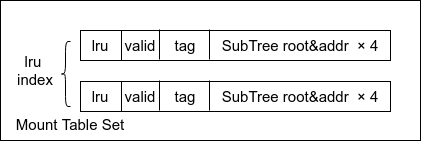
\includegraphics[scale=0.5]{Mount-Table-Set.png}
    \caption{\textbf{Mount-Table-Set }Mount Table缓存行中的数据结构}
   \label{fig:Mount-Table-Set.png}
\end{figure}
Mount Table Set中一个缓存行由四个部分组成,分别是lru bit,valid bit,tag,以及子树的根节点信息。其中lru bit记录了当前的缓存行最近是否被访问过,如果被访问锅则lru bit被设置为1,如果没有被访问过,则lru bit被设置为0.如果lru bit为0表示当前的缓存行能够被驱逐出去。valid bit表示当前的缓存是否有效,如果为1表示当前的缓存中的数据是有效的,可以被内存控制器之间读取。tag是用于区分相同缓存集合中不同的缓存行,只有tag匹配一直且valid bit为1才被人为是缓存命中。
一个缓存行中存储了四个子树的节点,其中每个子树根节点的大小为16B,包括了子树的counter以及地址。

在gem5的内存控制器中,通过$recvTimingReq(PacketPtr pkt)$接受来自cache的数据包,通过$port.schedTimingResp(pkt, response_time)$将读取的数据返还给cache。当内存控制器接受到数据包的时候,首先会检查对应内存是否需要完整性保护$checkSecureBItmap$,如果访问的内存不需要完整性保护则调用$recvTimingReqNonSecure(pkt)$,如果需要完整性保护则回去Mount Table中寻找对应的子树根节点,如果子树的根节点不在Mount Table中那么,会去MMT元素局区域获取
子树的根节点$acquireSubTreeNode(pkt)$,并且将从Mount Table中淘汰的子树的节点更新到MMT元数据区域中,同时更新Root-of-root的数值。当子树的根节点在Mount Table中,内存控制器能够进行之后的完整性检查。首先内存控制器会检查该数据包包含的内存访问是读请求还是写请求:$pkt->isWrite()$,$pkt->isWrite()$,如果是读请求,则将数据包放入内存控制器中的读缓存队列中,如果是写请求,则将数据包放入写缓存队列中。当数据包在读缓存队列中的时候,回去检查之前的
写缓存队列中是否存在相同内存地址的写请求,如果存在,那么可以直接将写请求中的数据放入读请求的数据包中,返回给cache。如果读请求的数据包对应的内存地址不在写缓存队列中,那么将会发起一次内存的读操作。为了保证内存中数据的完整性,我们还需要读取对应内存的子树中的节点。我们首先会去保存子树的节点的缓存中检查对应的子树节点是否在Tree Node Cache中,如果在Tree Node Cache中那么可以直接读取到对应的子树节点中的counter和hash(会根据子树的层数以及内存的地址计算对应的counter在子树节点中的offset),
如果不在Treee Node Cache中,则需要额外做一次内存的访存请求。所有的内存读写请求都会生成一次事件,加入到事件的调度其中。当读写内存请求的事件被调度到时,内存控制器会调用$processRespondEvent()$处理从内存中读到的数据。首先内存控制器会区分读取的数据是子树节点中的数据还是原本内存请求中的数据。当所有的子树节点中都在内存控制器中可读到时候(要么在Tree Node Cache中,要么从内存中读取出来),内存控制器会进行根据子树的节点对内存中的数据做完整性检查。
如果完整性检查成果,则内存中的数据写到数据包中,调用$port.schedTimingResp(pkt, response_time)$,将结果返回给cache。对于数据包中的请求是写请求的话,将数据包加入写缓存队列,并将写内存事件加入事件调度器中,内存控制器会去更新对应子树中counter值,然后通知cache,内存写请求更新完成。因为一旦数据包静茹了写队列,之后的读求情都会先在写队列中寻找是否存在对应的数据,写队列的中的数据包也会异步的刷到内存中。

\chapter{测试与评估}

\section{Benchmark测试}
下面我们将实现的MMT内存完整性保护原型,在SPECCPU和STREAM的测试集上进行测试。SPECCPU是一个标准的cpu,内存和io的综合测试,它选取了多个一个典型的应用场景,能够较好的反应机器的综合性能。STREAM是一个测试内存性能的测试集,有较大的内存压力,能够评估内存在极限情况的下的性能。
我们对比了不做任何完整性保护,使用SIT对内存进行完整性保护,使用vault对内存进行完整保护和使用MMT对内存进行完整性保护,在不同的测试集下的性能,同时页分析了页交换和Mount操作占总运行时间的比例,下面我们将具体的介绍每一个测试的结果。

\begin{figure}[!htp]
    \centering
    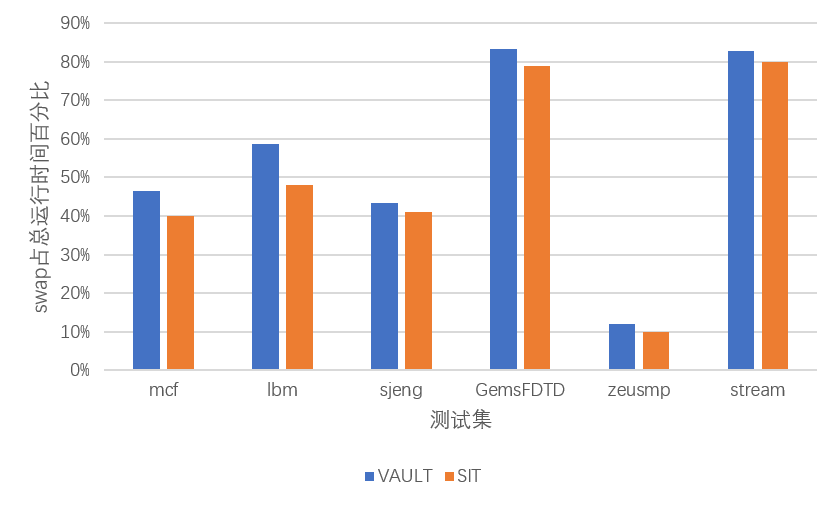
\includegraphics{eval-swap.png}
    \caption{\textbf{SPECCPU, STREAM测试集在不同完整性保护方案下swap所占比列}。}
   \label{fig:eval-swap}
\end{figure}
如图 ~\ref{fig:eval-swap}所示,我们分别测试了SIT,VAULT等先进的完整性保护方案,在超过soc上保护内存限制时候产生swap的开销占总运行时间的比例。为了能够理论上支持无限制的内存完整性保护方案,在SIT以及VAULT等方案中一旦使用的内存超过了soc可以保护的范围。CPU会选择恰当
页将其中改的数据进行加密,然后swap到非安全的内存中。为了保证从非安全内存中swap回到安全内存中,数据没有被修改。CPU在swap的时候会生成一个evict metatdate结构。该结构中记录了swap出去页的哈希值,以及属于哪一个enclave等相关的元数据,该结构被存储在安全内存中。注意当安全内存
十分紧张的时候,该数据结构也可能被swap到非安全内存中,同样我们会为存放evict metadata的页生成一个evict metadata,类似于树的形式,只需要保存根上的evict metadata既可以保证所有swap出去页的完整性。虽然SIT,vault能够理论上支持更多的内存,但是当SoC上保护得内存耗尽的时候
swap会带来很严重的性能开销,测试发现,一次swap将会带来高达40k的开销,我们在SPECCPU和STREAM测试集上进行了测试(这里我们挑选了SPECCPU中运行时内存超过128M的测试用例),我们发现swap占据了总运行时间的10\%-80\%,其中5/6的测试结果显示swap占据了总运行时间的40\%以上,其中GemsFDTD和STREAM测试swap的开销格外严重,占据了总运行时间的80\%以上,
另外杜比SIT和VAULT,在VAULT中swap的开销会更加的严重,这不是应为VAULT的设计的缺陷,还是因为VAULT运行时候的气态开销更小,导致了swap所占的时间更加明显。通过上面的数据显示,一旦使用的内存超过了SoC上保护的限制,swap将造成验证的性能降级,所以优化swap的开销非常的重要。

\begin{figure}[!htp]
    \centering
    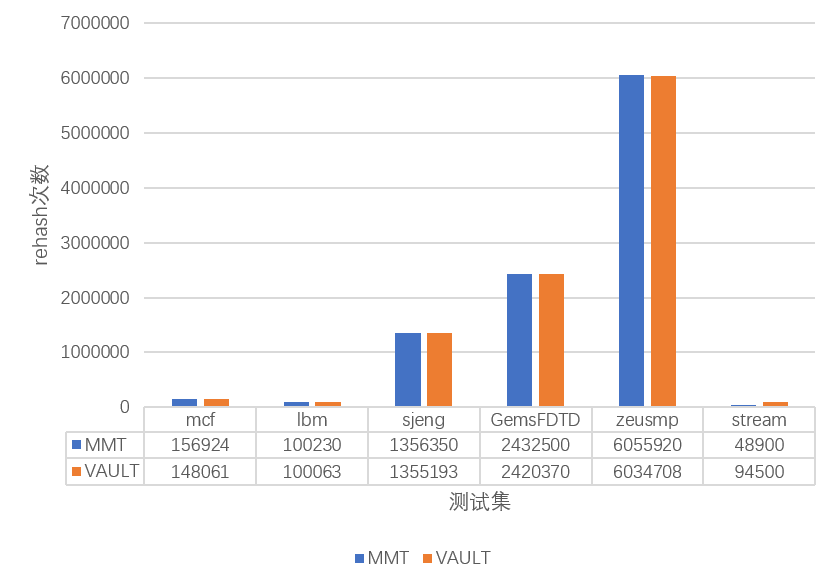
\includegraphics{eval-rehash.png}
    \caption{\textbf{SPECCPU, STREAM测试集在不同完整性保护方案下rehash的次数}。}
   \label{fig:eval-rehash}
\end{figure}
如图 ~\ref{fig:eval-rehash}所示,我们测试了VAULT和MMT中rehash的次数。为了能够增加完整性保护树中节点的扇出,VAULT和MMT都采用了分级counter的设计思路。因为分级counter会带来rehash的额外开销,来缓解replay等攻击。在MMT的设计中我们采用了三级counter的设计,三级counter的设计充分考虑了
完整性保护树中的冷热counter不均衡,在较高的树节点中往往只存在一个活跃的counter,而其他的counter可能处于不活跃的状态,所以我们可以减少冷counter比特数,增加热counter的比特数,从而兼顾安全性于节点的扇出。在这里我们同先进的VAULT完整性保护方案进行了比较。其中VAULT的稳定扇出为24,而MMT中
节点的扇出为32。在更大的扇出情况下,MMT并没造成更多的rehash的次数,说明在真实的workload下,完整性保护树中的冷热counter分布不均衡,而extra counter的设计能够很好的考虑到这种情况,从而进一步的提高树节点的扇出。在SPECCPU的测试集中,大多数的场景下,MMT于VAULT的rehash的次数相差小于1\%,
在stream的场景中,因为内存访问的比较规律,同时使用的内存较少,通过extra conter的方式能够使热counter拥有更多的比特数,从而减少热counter rehash带来的影响。所以相较于VAULT而言rehash的次数反而更少了。综上,我们认为MMT三层counter的设计充分考虑了完整性保护树的不均衡性,在实际场景中不会带来更多的
开销,在个别场景中,会比先经的VAULT的rehash开销更少。

\begin{figure}[!htp]
    \centering
    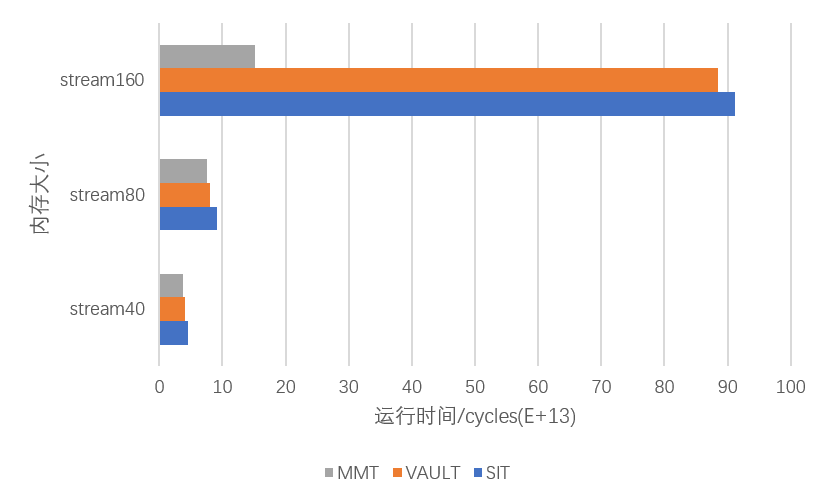
\includegraphics{eval-memorysize.png}
    \caption{\textbf{STREAM测试集使用内存大小与不同完整性保护方案下性能关系图}。}
   \label{fig:eval-memorysize}
\end{figure}
如图 ~\ref{fig:eval-memorysize}所示,我们比较程序使用不同的内存大小,对完整性检查的影响,在这里我们选取了STREAM测试集。STREAM是为了测试内存的性能的测试集,拥有较大的内存压力,频繁的读写内存能够快速耗尽SoC上能保护得安全内存得空间,同时产生频繁得swap操作。这里我们分别选取了SIT, VAULT, MMT对使用40M, 80M, 160M内存
得STREAM测试集做了分析。当程序使用的内存少于SoC上能够保护得内存时候,SIT,VAULT,MMT之间得差距并不是很明显。SIT会比MMT慢20\%左右,和VAULT相比,MMT采用了三级counter得设计,与VAULT相相比略有性能提升。因为40M和80M得内存较少,没有充分发挥三级counter得优势,当进一步扩大内存得时候三级counter得优势会更加的明显。
当使用的程序使用的内存超过了128M得时候。SIT和VAULT得性能开销急剧增加,因为STREAM会频繁循环的的访问内存,所以一旦超出了SoC上能够保护的内存时,就会频繁的发生swap操作,造成较大的性能开销。和SIT,VAULT相反,MMT采用了挂挂载的方式代替内存的swap,挂载操作的开销非常小(100~200 cycles)。所以当使用的内存扩大了一倍,
运行时间也线性的扩大了一倍,挂载操作并没有成为性能的瓶颈。而swap操作会带来7,8倍的性能开销,说明swap操作取代了完整性保护的检查,成为了主要的瓶颈。

\begin{figure}[hbt]
    \centering
    \setlength{\belowcaptionskip}{0pt}
    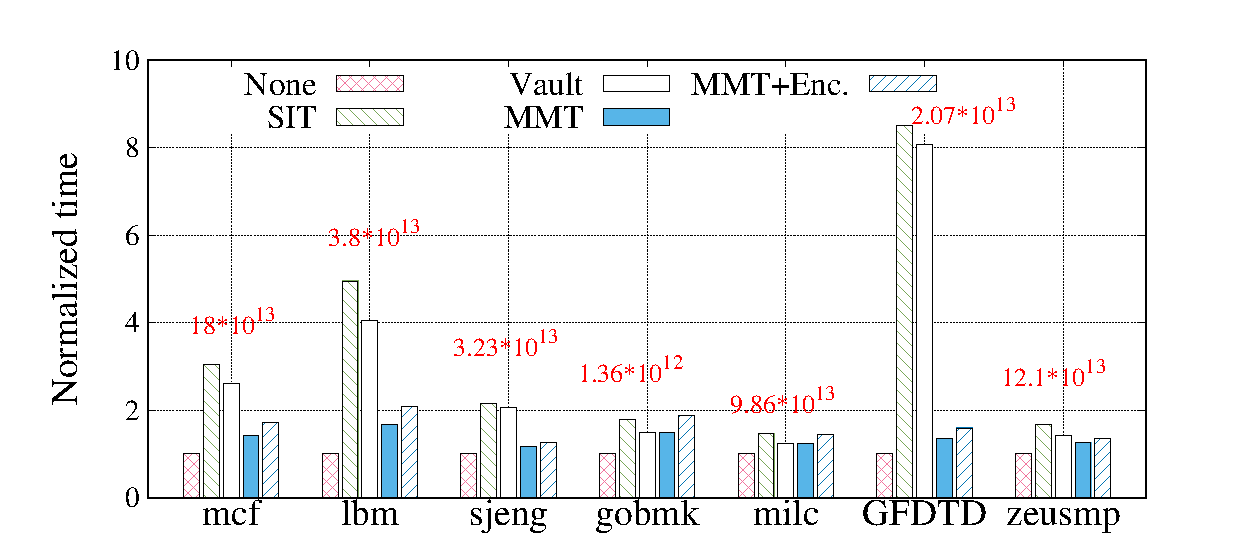
\includegraphics[scale=0.6]{fig/eval-integrity-bench.eps}
    \caption{\textbf{SPECCPU测试集在不同完整性保护方式下的性能}. \emph{None} 表示没有完整性保护下的理论性能。}
    %Compared with SGX and Vault, {\forest} can achieve the best performance in all the cases.
    \label{fig:eval-inter-bench}
\end{figure}
如图~\ref{fig:eval-inter-bench}所示,我们在SPECCPU上测试了SIT, VAULT, MMT, MMT+encrypt, 以及不做完整性检查原始的测试。其中\emph{gobmk},\emph{milc}两个测试集使用的内存小于128M,不会产生swap的开销,剩下的测试程序使用的内存从[180M:1200M]不等。从测试结果中我们可以发现,MMT的性能均优于SIT和VAULT,
在mcf的测试中,SIT和VAULT相较于没有完整性保护的程序分别会有2.05x和1.6x的开销,而MMT只有0.4x的开销,这部分的开销主要是完整性检查的开销,而挂载的开销小于1\%(挂载的操作只需要100~200的开销),在其他的测试中例如GemsFDTD,SIT和VAULT相较于不做完整性检查的程序来说有高达7.5x和7.06x倍的性能开销,而MMT只会
有0.35x的性能的开销。在这种极限的场景下,MMT相较于没有完整性保护的原程序来说只有0.35x的开销,Mount操作大幅减少了原有的swap的开销,并且在绝大多数的场景下,Mount的开销可以忽略不记(<1\%)。当使用内存小于SoC上可以保护的内存时候,MMT和Vault相比性能相近(这里为了是SoC上保护的内存相同,我们减少了MMT树的个数,因此三级counter的优势没有很好的体现)。
根据上面的测试我们可以得出,不论在内存使用超过SoC能保护的内存大小,还是小于SoC保护的内存时候,MMT都具有最好得性能,特别是当使用得内存超过SoC保护得内存大小得时候,挂载操作将极大得缓减原本swap页所带来的开销,又因为在运行时,可以通过Mount Table中读取子树的根节点来保证运行时候对完整性树检查的层数不变,从而保证SoC上内存足够的情况下,也不会带来额外的开销。

\section{性能评估}
通过以上的测试结果我们发现,对于传统的页交换操作,当使用的内存操作了SoC上能够保护内存大小的时候,会带了及其严重的性能开销,在极端的场景下,能够达到近十倍的性能下降。如此大的性能开销是完整性保护系统不可以接受,这也是为什么已有sgx的应用会指明使用的内存应该小于128M(EnclaveDB)。而对于挂载(Mount)操作,在最严重的场景下,其开销不会超过1\%,因为Mount带来的
开销相较于完整性检查可以忽略不计。因为Mount的存在,我们不需要在SoC中保护所有的内存,而只需要保护当前活跃的数据。因为内存访问的局域性,程序某一个时间段内存访问的内存将远小于它总共使用的内存,因此将大多数的子树放在内存是可行的,同时也是的MMT能够保护的内存大小达到TB级别。MMT不仅能够将保护的内存范围扩大几个数量级,同时也能够实现可扩展的内存分配,离散的内存保护。
在传统得完整性保护树中,只能够保护一块连续的固定的内存空间,并不能够动态的扩展该内存大小,同时也无法保护离散的内存区域。这些缺陷都限制了内存完整保护的可扩展性,并不是适应于云场景的环境。MMT的提出使得云场景中内存完整性保护成为了可能,结合内存隔离与加密技术,能够实现内存强安全保障。

MMT的性能也会受到以下几个因素的影响。一、虽然MMT支持离散内存的完整保护,但是在个别离散的场景中,会带来较大的性能开销。例如在每一颗一个子树中,只保护一页大小的内存完整,如果有一个程序恰好使用这些内存,那么每次的访问都有可能产生Mount与Unmount操作,从而带来较大的性能开销。然后在真实的场景中,这样的内存访问模式是很难产生的,因为程序具有一定的局域性,并且操作
系统也能够辅助,将程序使用的内存都分配在一起,缓解内存过于离散造成的频繁的挂载与卸载操作。二、在多核多cpu的场景下,为了保证每一个核至少有一个子树能够使用,Mount Table中保存的子树的个数应该至少超过cpu中的核数,这样才能够保证不会出现不同的核相互卸载其他核正在使用的子树。我们认为,Mount Table的大小应该是和核数成正相关,在多核的场景下,SoC上也会有更多的空间,
用于存储必要的信息。三、Mount操作在极端的场景中可能比页交换的次数还要多,例如程序对内存的访问刚好只访问子树中的个别几个页,从而导致频繁的子树切换。而对于页交换策略,因为只需要访问子树中的个别几个页,一段时间内使用的内存并不多,因此不会产生频繁的页替换。虽然页替换的次数可能小于挂载的次数,但是由于页交换需要40k cycles而Mount只需要100\sim200 cycles。所以Mount所花
的时间还是远小于页交换的时间。又因为一棵子树的大小为4M远大于页4K的大小,因此在一般的场景下,Mount操作的次数将远小于页交换的次数,结合Mount本身较少的操作时间,使得Mount所带来的开销几乎可以忽略不记。


% \input{tex/math_and_citations}
% !TEX root = ../thesis.tex

\begin{summary}
本文对内存完整性保护方案做了系统的分析,就内存完整性保护的大小,树中节点数据结构,危险模型与安全性分析做了仔细地探讨。通过对已有的内存完整性保护的研究发现,虽然已有的工作能够理论上实现
对GB级别的内存数据做完整性检查,但是任然不适合云场景中的TB级别的内存,以及安全内存的可扩展性。在本文中,我们提出了一种新颖的完整性保护数据结构:哈希森林以及可挂载完整性保护树。其中挂载的单位是子树,在MMT中子树还会处于三个状态:活跃,不活跃与未分配
并且针对子树的概念提出了两个新的动态操作:挂载(Mount)与卸载(Unmount)。本文通过这两个新增的完整性保护树的动态原语,实现了可扩展的内存完整性保护,动态的安全内存分配以及针对离散内存的保护。同时结合了内存访问的规律,
提出了三级counter的树节点架构,针对冷热counter做了进一步的优化,从而实现了在不影响安全性的前提下,增加了额树节点的扇出,扩大了内存保护的范围。

在论文中,实现了基于MMT完整性保护树,以及哈希森立的内存保护原型。通过在内存控制器中增加三个部件:Secure Bitmap;Mount Table;Root-of-root来实现子树的挂载,内存的完整性检查等操作。同时对内存中的布局就做进一步的细化,将内存区域分成了:非安全内存,
安全内存,子树区域与MMT元数据区域,为了保护MMT元数据区域内的数据不被攻击者篡改,我们才用了RISCV架构的M mode中monitor对该区域进行管理,同时采用pmp寄存器对MMT元素据区域进行隔离,保证特权软件无法篡改其中的子树的根节点。

在论文中,对针对内存的攻击进行了详细的分析与归类,并且通过密码学的方式证明了对内存完整性保护的可行性,同时也分析了不同数据结构可能带来的安全隐患。论文中详细分析MMT与VAULT, BMT等相关工作的安全性,虽然MMT采用了更加激进的counter组织方式,但是得益于对内存
访问pattern的观察,MMT会比VAULT有更强的安全性(更低的概率实现重放攻击)。之后的测试也表明,MMT所采用的树的数据结构并不会带来更多的运行时开销。

在实现中,对于树的配置:MMT子树的层数为3,保护的内存为4M,根树的层数时3,保护的内存为2M;SoC上的开销:Secure Bitmap大小为16K,Mount Table大小为512B;内存开销:MMT元数据区域大小约为2M。在极少的完整性保护树的层数下(<SGX的6层),极少了SoC空间开销的情况下(16Kb空间),我们实现了
对512G的内存数据的完整性保护,同时可有SoC保护的内存为128M。针对不同的情况,可以增加树的层数,以及Mount Table的容量,实现更多内存的完整性保护。

论文基于gem5模拟器实现了VAULT,SGX,MMT等多种内存完整性保护方案。首先我们测试了传统的交换页的机制对性能的影响,测试结果表明,交换页对占总运行时间的百分之40以上;其次我们测试在极限场景下,传统完整性保护方案的开销(7\sim8倍的开销);最后我们基于SPECCPU对MMT和其他完整性保护方案进行了对比,
MMT均取得了最好的性能且Mount操作带来的额外开销小于1\%,保证了内存完整性保护的可扩展性。
\end{summary}


% 使用英文字母对附录编号
\appendix

% 附录内容,本科学位论文可以用翻译的文献替代。
% \input{tex/app_maxwell_equations}
% \input{tex/app_flow_chart}

% 文后无编号部分
\backmatter

% 参考资料
\nocite{*}
\printbibliography[heading=bibintoc]


% 用于盲审的论文需隐去致谢、发表论文、参与项目、申请专利、简历

% 致谢
% !TEX root = ../thesis.tex

%TC:ignore

\begin{acknowledgements}
  感谢我的毕业设计的老师夏虞斌副教授对我论文的指导与帮助!

  感谢上海交通大学软件学院的各位老师四年来对我的辛勤教育和专业技能上的培养!

  感谢16级软件学院的同学们四年来对我的帮助与鼓励,让我度过了一个愉快而又充实的大学四年时光

  感谢我的父母,这几十年来对我的养育之恩以及辛勤的教导,在我最困难的时候给予我最打的鼓励,感谢你们
\end{acknowledgements}

%TC:endignore


% 发表论文、参与项目、申请专利、简历
% 盲审论文中,发表学术论文及参与科研情况等仅以第几作者注明即可,不要出现作者或他人姓名
% \input{tex/publications}
% \input{tex/projects}
% \input{tex/patents}
% \input{tex/resume}

% 中文学士学位论文要求在最后有一个英文大摘要,单独编页码,英文学士学位论文不需要
% !TEX root = ../thesis.tex

\begin{bigabstract}
  In this paper, we proposes a new integrity tree organization, Mountable Merkle Tree (MMT). MMT promises a stable tree depth which will not increase with total memory size, and minimize the memory overheads by storing integrity metadata 
  (hashes and counters) on demand. We leverages MMT for the scalable memory integrity protection.

  Traditional integrity trees use a single tree to manage the hashes and counters for all data. That means the size (or depth) will increase along with the secure memory size, e.g., protecting 512GB memory in SGX needs an 11 depth integrity tree. Instead, 
  MMT introduces a new concept, hash forest which includes a set of integrity trees protecting different memory regions. We call a single tree in the forest as SubTree. Each SubTree protects a fixed size memory region, e.g., 4MB in our design.

  With the limited space in the SoC, MMT puts all the SubTrees in the memory. MMT uses a RootTree to protect the integrity of all in-memory SubTrees.
  The common root ancestor of RootTree is fixed in the SoC (i.e., the Root-root) to prevent attacks. The RootTree can dynamically add or remove a
  SubTree from the hash forest. The mounted SubTrees represent the hot set of memory, which can boost integrity checking performance. When memory augments, MMT need not increase the SubTree depth but add more SubTrees in the forest. For each secure memory accesses, MMT will first check
  whether the SubTree of accessed address is mounted. If it is, MMT checks the integrity using the in-SoC SubTree like traditional approaches. Otherwise MMT uses a mounting mechanism to mount the target SubTree into the SoC.

  \textbf{Mounting.} The storage space for mounting SubTrees root in
  the SoC is restricted, e.g., MMT allows 32 subtrees simultaneously. When space is exhausted, MMT unmounts the
  inactive SubTree root out of the SoC and stores it in memory,
  which is isolated with host memory in DRAM. Meanwhile,
  MMT needs to update the value of the ancestors if necessary.
  With the conception of the hash forest, MMT can realize on-demand memory integrity protection, and support the
  integrity protection of discrete physical memory.

  \textbf{Integrity checking.} MMT will always enable integrity
  protection when executing in the monitor (i.e., when executing in machine mode). As an enclave can access both
  secure and non-secure memory (untrusted sharing memory),
  we can not just impose integrity protection on all its pages.
  In addition, protecting all enclaves is not suitable as some
  enclaves do not care about integrity protection and prefer
  better performance. MMT introduces two kinds of
  registers, mode status register (Reg\_MS) and hole registers
  (Reg\_hole\_VA\_start and Reg\_hole\_VA\_size) to resolve the
  issues. Reg\_MS represents whether the current CPU needs integrity protection, so the monitor can meet different integrity
  needs for distinct enclaves by controlling Reg\_MS. The hardware will apply integrity protection to all pages current CPU
  uses when $MS== 1$ (i.e., executing enclave) and disable it
  when $MS== 0$ in general. Hole registers are used to represent
  a special virtual memory region that the integrity checking
  is enabled when $MS== 0$ or disabled when $MS== 1$, e.g.,
  enclave can share the untrusted memory with host in the hole
  region that won't need integrity protection.

  \textbf{Bootstrap.} In the hardware extension of
  MMT. Besides the untrusted normal memory, there are three
  regions, secure memory (enclaves and monitors), SubTree
  nodes, and MMT meta-zone. Only the MMT meta-zone is a
  fixed region configured by hardware bootrom, and the size of
  the MMT meta-zone is 2.14MB (supports 512GB memory).
  During system boot, the bootrom will initialize the MMT
  meta-zone and allocate the subtree nodes for the monitor
  memory. Then the monitor is loaded with integrity protection
  and now takes the responsibility to manage integrity.

  \textbf{SubTree allocation.} Not all physical memory needs integrity
  protection (e.g., kernel memory), so it will not allocate all
  SubTree nodes at the bootstrap. However, the monitor needs
  to allocate memory for the subtree nodes when new memory
  regions are changed to secure memory and sets the SubTree
  root and address in the MMT meta-zone. As MMT meta-zone
  can only be accessed by monitor, no others can tamper the
  SubTree allocation.

  We evaluate the MMT, SIT, VAULT on SPECCPU and STREAM benchmarks. The test results indicate that the page swap mechanism adopted in the SGX will bring serious performance overhead. Page swapping can occupy the 40\% proportion runtime in most benchmark cases, and may lead to 7 \sim 8 times performance overhead in the extreme case. We propose the MMt to mitigate the page swapping overhead with the dynamic primitives for integrity tree: Mount and Unmount. Mount and unmount only take 200 hundreds to fetch the subtree root and address from the MMT metadata zone and mount it in the Mount table in memory controller. The preliminary tests running on SPECCPU demonstrate that the extra overhead for mount and unmount operation is less than one percent, which is negligible in the most case. Comparing with SIT and VAULT, MMT demonstrates 2 to 3 times speed up, and the dominating overhead is integrity checking, fetching the tree node and computing the hash or mac for each  node and original data. We adopt the three level counter structure in each subtree node, which promotes the fan out up to 32. The depth of subtree is limited to 3, which can protect 4M memory. If SIT wants to protect the same size of memory, it need 5 levels of tree nodes. With the benefit of MMT tree node structure, we can further mitigate the runtime overhead for memory integrity protection. 

In our prototype, MMT can protect up to 512G memory with 3-level subtree structure, which is more capable than SIT that can only protect 128M memory. All the tree node data and mac can be dynamically allocated later, the only fixed zone in the memory space when machine startup is MMT metadata zone, which is only about 2M. The memory overhead and runtime overhead is acceptable to support scalable memory integrity protection. 

\end{bigabstract}


\end{document}
